\documentclass[11pt, a4paper]{article}

% --- PACOTES PRINCIPAIS ---
\usepackage[utf8]{inputenc}
\usepackage[T1]{fontenc}
\usepackage[brazil]{babel}
\usepackage{lmodern}
\usepackage{geometry}
\geometry{a4paper, top=2.5cm, bottom=2.5cm, left=2.0cm, right=2.0cm}
\usepackage{amsmath, amssymb, amsfonts}
\usepackage{booktabs}
\usepackage{tabularx}
\usepackage{graphicx}
\usepackage{xcolor}
\usepackage{enumitem}
\usepackage{tcolorbox}
\usepackage{fancyhdr}
\usepackage{float}
\usepackage{caption}
\usepackage{tikz}
\usetikzlibrary{positioning, arrows.meta}
\usepackage[colorlinks=true, linkcolor=ufopred, citecolor=deepnavy, urlcolor=ufopred]{hyperref}

\graphicspath{{figures/}}

% --- CORES INSTITUCIONAIS UFOP ---
\definecolor{ufopred}{RGB}{140, 29, 36}
\definecolor{deepnavy}{RGB}{20, 35, 60}
\definecolor{lightgray}{RGB}{245, 247, 250}
\definecolor{darkslate}{RGB}{30, 40, 50}

% --- CONFIGURAÇÃO DE CABEÇALHO E RODAPÉ ---
\pagestyle{fancy}
\fancyhf{}
\setlength{\headheight}{14pt}
\rhead{\textcolor{darkslate}{\small \textbf{BCC327 -- Computação Gráfica} --- TP1}}
\lhead{\textcolor{darkslate}{\small Visualização, Rasterização e Recorte de Árvores CCO}}
\cfoot{\thepage}

\tcbuselibrary{skins, breakable}
\captionsetup{font=small, labelfont=bf}

\begin{document}

% --- TÍTULO E AUTORES ---
\begin{center}
  {\LARGE \bfseries \textcolor{ufopred}{Visualização Geométrica, Rasterização e Recorte de Árvores Arteriais Geradas pelo Método CCO}}\\[0.4cm]
  {\large \textbf{Heitor Augusto de Oliveira Ramos}$^{1}$, \textbf{Rafael Stylita Duarte}$^{1}$}\\[0.2cm]
  {\small $^{1}$Departamento de Computação (DECOM) --- Universidade Federal de Ouro Preto (UFOP)\\[0.1cm]
  Trabalho Prático 1 --- BCC327 Computação Gráfica --- 2026.2 --- Prof. Dr. Rafael Alves Bonfim de Queiroz}\\[0.4cm]
\end{center}

% --- CAIXA DE RESUMO E PALAVRAS-CHAVE ---
\begin{tcolorbox}[colback=lightgray, colframe=deepnavy, arc=3pt, title=\textbf{RESUMO}, fonttitle=\bfseries]
\small
\textbf{Contexto:} Árvores arteriais sintéticas geradas pelo método \emph{Constrained Constructive Optimization} (CCO) são distribuídas em arquivos VTK que guardam apenas pontos, conectividade e o raio de cada vaso; transformar esses dados em imagem exige todas as etapas clássicas do \emph{pipeline} gráfico.
\textbf{Objetivo:} Desenvolver uma aplicação única que leia, represente, transforme, rasterize e recorte os modelos CCO 2D e 3D fornecidos, deixando explícito o que é implementação própria e o que vem da biblioteca.
\textbf{Metodologia:} Em Python, implementamos um leitor de VTK ASCII, matrizes homogêneas $4\times4$, Bresenham, \emph{Scanline Fill} com tabelas de arestas, supersampling por cobertura, Cohen--Sutherland, Liang--Barsky e Sutherland--Hodgman. A renderização interativa (tubos, câmera, projeções, MSAA/SSAA) usa PyVista/VTK.
\textbf{Resultados:} Os dois modelos (128 pontos, 127 segmentos cada) são exibidos como tubos com cor e espessura proporcionais ao raio. O supersampling $4\times4$ reduz em cerca de 11 vezes o erro de cobertura de uma reta inclinada em relação à amostragem simples. Cohen--Sutherland e Liang--Barsky produzem recortes idênticos nos 127 segmentos; o primeiro resolve 114 deles trivialmente e calcula apenas 14 interseções.
\textbf{Conclusão:} Os sete módulos do enunciado foram atendidos; o caso côncavo do Sutherland--Hodgman evidencia quando o Weiler--Atherton é necessário.

\vspace{0.2cm}
\textbf{Palavras-Chave:} Computação Gráfica; Método CCO; Rasterização; Antialiasing; Recorte; VTK.
\end{tcolorbox}

\vspace{0.4cm}

% =====================================================================
\section{Introdução}
% =====================================================================
A simulação de escoamento sanguíneo e o estudo da perfusão de tecidos dependem de representações geométricas da árvore vascular. Como imagens médicas não resolvem os vasos mais finos, modelos sintéticos são uma alternativa. O método CCO, introduzido por Schreiner e Buxbaum~\cite{schreiner1993}, constrói essas árvores adicionando um segmento terminal por vez e otimizando a posição de cada nova bifurcação sob restrições fisiológicas.

Uma árvore CCO, porém, é apenas um conjunto de números: coordenadas de pontos, pares de índices e um raio por segmento. Para que ela se torne uma imagem, é preciso escolher primitivas, mapear atributos em cor, posicionar o observador, projetar, converter a geometria contínua em pixels e descartar o que está fora da área de visualização. Este trabalho percorre essas etapas com os modelos \texttt{tree2D\_Nterm064.vtk} e \texttt{tree3D\_Nterm064.vtk} fornecidos pelo professor.

\textbf{Objetivos.} Construir uma aplicação que (i) leia e interprete os modelos VTK; (ii) represente a árvore por tubos com cor e espessura em função do raio; (iii) aplique translação, rotação e escala e ofereça diferentes vistas e projeções; (iv) implemente Bresenham e \emph{Scanline Fill}; (v) compare imagens com e sem antialiasing; (vi) implemente e compare Cohen--Sutherland e Liang--Barsky; e (vii) implemente Sutherland--Hodgman e discuta o Weiler--Atherton. A Seção~\ref{sec:fund} resume a teoria, a Seção~\ref{sec:metodo} descreve a arquitetura, a Seção~\ref{sec:result} apresenta os resultados e a Seção~\ref{sec:disc} discute limitações e escolhas.

% =====================================================================
\section{Fundamentação Teórica}\label{sec:fund}
% =====================================================================

\subsection{Árvores CCO e o formato VTK}
No CCO, a árvore cresce dentro de um domínio de perfusão: cada novo terminal é conectado ao segmento que minimiza uma função de custo (tipicamente o volume total), e os raios são reajustados para manter pressões e fluxos consistentes~\cite{schreiner1993}. Neste trabalho não regeramos as árvores: usamos os modelos prontos, cada um com $N_{term}=64$ terminais, 128 pontos e 127 segmentos. Os arquivos estão no formato VTK legado ASCII, \texttt{DATASET POLYDATA}: a seção \texttt{POINTS} lista as coordenadas $(x,y,z)$, a seção \texttt{LINES} lista cada segmento como \texttt{2 id\_início id\_fim}, e \texttt{CELL\_DATA} traz o escalar \texttt{raio}, um valor por segmento~\cite{vtk}.

\subsection{Transformações geométricas e observador}
Em coordenadas homogêneas, o ponto $\mathbf{p}=(x,y,z,1)^T$ é transformado por matrizes $4\times4$, e translações passam a ser produtos de matrizes como as demais transformações~\cite{foley,hearn}:
\begin{equation}
T(\mathbf{d})=\begin{bmatrix}1&0&0&d_x\\0&1&0&d_y\\0&0&1&d_z\\0&0&0&1\end{bmatrix},\quad
S(s)=\begin{bmatrix}s&0&0&0\\0&s&0&0\\0&0&s&0\\0&0&0&1\end{bmatrix},\quad
R_z(\theta)=\begin{bmatrix}\cos\theta&-\sin\theta&0&0\\\sin\theta&\cos\theta&0&0\\0&0&1&0\\0&0&0&1\end{bmatrix}.
\end{equation}
Para girar ou escalar em torno de um pivô $\mathbf{c}$ (o centroide da árvore), usa-se $M' = T(\mathbf{c})\,M\,T(-\mathbf{c})$, e a matriz acumulada é $M_{acc} \leftarrow M' M_{acc}$.

\textbf{Espaço do mundo $\times$ sistema da câmera.} As coordenadas do VTK, depois das transformações de modelagem, estão no \emph{espaço do mundo}, comum a todos os objetos da cena. A câmera é definida por posição $\mathbf{e}$, ponto focal $\mathbf{f}$ e vetor \emph{up}. Com eles se monta uma base ortonormal $(\mathbf{u},\mathbf{v},\mathbf{w})$, com $\mathbf{w}=(\mathbf{e}-\mathbf{f})/\|\mathbf{e}-\mathbf{f}\|$, e a matriz de visualização leva cada ponto do mundo para o \emph{sistema da câmera}, onde o observador está na origem olhando ao longo de $-\mathbf{w}$~\cite{angel}. Transformar o modelo muda as coordenadas dos pontos no mundo; mover a câmera muda apenas essa mudança de base. Na aplicação as duas operações são separadas: as teclas de transformação alteram os pontos, e as teclas de vista alteram a câmera.

\textbf{Projeções.} Na projeção ortográfica os projetores são paralelos e tamanhos não dependem da profundidade ($x_p=x_c$, $y_p=y_c$). Na perspectiva, os projetores convergem no centro de projeção e $x_p = d\,x_c/(-z_c)$, $y_p = d\,y_c/(-z_c)$: objetos mais distantes aparecem menores.

\subsection{Rasterização}
\textbf{Bresenham.} Para uma reta no primeiro octante ($0\le m\le1$), em cada coluna $x$ escolhe-se entre o pixel $(x+1,y)$ e o $(x+1,y+1)$ pelo sinal de uma variável de decisão atualizada só com somas inteiras~\cite{bresenham1965}. Usamos a forma generalizada para os oito octantes, com erro $e = \Delta x - \Delta y$ e $e_2 = 2e$: se $e_2 > -\Delta y$ avança-se em $x$, e se $e_2 < \Delta x$ avança-se em $y$. São gerados $\max(|\Delta x|,|\Delta y|)+1$ pixels com conectividade de 8 vizinhos. O DDA chega ao mesmo resultado, mas usa divisão e arredondamento em ponto flutuante a cada passo.

\textbf{Scanline Fill.} Cada aresta não horizontal entra na Tabela de Arestas (ET), indexada pela primeira linha inteira que cruza, com $y_{fim}$ e o incremento $1/m=\Delta x/\Delta y$. Para cada linha $y$, a Tabela de Arestas Ativas (AET) recebe as arestas que começam, perde as que terminam, é ordenada por $x$, e os pixels entre pares consecutivos de interseções são preenchidos (regra par-ímpar). Depois, cada $x$ é atualizado incrementalmente com $x \leftarrow x + 1/m$. O intervalo semiaberto $[y_{min}, y_{max})$ de cada aresta impede que um vértice compartilhado seja contado duas vezes.

\subsection{Aliasing e antialiasing}
Amostrar uma primitiva contínua com uma única amostra por pixel produz \emph{aliasing}: bordas em degrau e vasos finos que somem ou se fragmentam quando sua largura é menor que um pixel. O \emph{supersampling} (SSAA) avalia $k\times k$ amostras por pixel e usa a fração coberta como intensidade, aproximando a integral de cobertura do pixel. O MSAA, usado pelas GPUs, guarda várias amostras de cobertura e profundidade por pixel, mas avalia a cor uma única vez por primitiva; por isso suaviza as bordas geométricas com custo menor que o SSAA, mas não trata o aliasing interno das texturas e do sombreamento.

\subsection{Recorte de segmentos}
\textbf{Cohen--Sutherland}~\cite{foley}. Cada extremo recebe um código de 4 bits (acima, abaixo, direita, esquerda da janela). Se $c_0 \lor c_1 = 0$, o segmento é aceito trivialmente; se $c_0 \land c_1 \neq 0$, os dois extremos estão do mesmo lado de fora e o segmento é rejeitado trivialmente. Caso contrário, um extremo de fora é movido para a interseção com uma borda e o teste se repete.

\textbf{Liang--Barsky}~\cite{liang1984}. Com $P(u)=P_0+u\,(P_1-P_0)$, $0\le u\le1$, as quatro condições de pertinência são escritas como $p_k u \le q_k$, com $p=(-\Delta x, \Delta x, -\Delta y, \Delta y)$ e $q=(x_0-x_{min},\, x_{max}-x_0,\, y_0-y_{min},\, y_{max}-y_0)$. Se $p_k<0$ o segmento entra pela borda $k$ e $u_1=\max(u_1, q_k/p_k)$; se $p_k>0$ ele sai e $u_2=\min(u_2,q_k/p_k)$; se $p_k=0$ e $q_k<0$ o segmento é paralelo à borda e está fora. O trecho visível é $[u_1,u_2]$, se $u_1\le u_2$. Cada extremo é calculado uma única vez, sem as interseções intermediárias do Cohen--Sutherland.

\textbf{Cyrus--Beck (discutido, não implementado)}~\cite{cyrus1978}. Usa a mesma ideia paramétrica, mas para uma janela \emph{convexa qualquer}: para cada aresta $i$ da janela com normal interna $\mathbf{N}_i$ e um ponto $\mathbf{E}_i$ sobre ela, resolve $\mathbf{N}_i\cdot(P(t)-\mathbf{E}_i)=0$ e classifica $t$ como entrada ou saída pelo sinal de $\mathbf{N}_i\cdot(P_1-P_0)$. A principal diferença é a janela: Cohen--Sutherland e Liang--Barsky exigem um retângulo alinhado aos eixos (códigos de região e as quatro comparações fixas), enquanto Cyrus--Beck aceita qualquer polígono convexo, ao custo de produtos escalares por aresta. Liang--Barsky é exatamente o Cyrus--Beck com normais $(\pm1,0)$ e $(0,\pm1)$.

\subsection{Recorte de polígonos}
\textbf{Sutherland--Hodgman}~\cite{sutherland1974}. O polígono é recortado sucessivamente contra o semiplano interno de cada aresta da janela convexa. Para cada aresta $(S,E)$ do polígono há quatro casos: dentro$\to$dentro emite $E$; dentro$\to$fora emite a interseção; fora$\to$dentro emite a interseção e $E$; fora$\to$fora não emite nada. A saída é sempre \emph{uma única} lista de vértices.

\textbf{Weiler--Atherton (discutido)}~\cite{weiler1977}. Calcula as interseções entre as fronteiras do polígono e da janela, insere-as nas duas listas de vértices marcadas como entrada ou saída e percorre as listas alternando entre polígono e janela a cada interseção. Por isso pode devolver \emph{várias} regiões separadas e aceita janelas côncavas e polígonos com buracos. É o algoritmo adequado quando o polígono é côncavo e o recorte o divide em mais de uma região (a saída do Sutherland--Hodgman ligaria as regiões por arestas sobrepostas ao longo da borda da janela), quando a própria janela é côncava, quando há buracos ou várias regiões, e em operações booleanas entre polígonos (união, interseção, diferença). O custo é uma implementação mais complexa, com casos especiais para vértices sobre arestas e interseções tangentes.

% =====================================================================
\section{Metodologia e Arquitetura da Aplicação}\label{sec:metodo}
% =====================================================================
A aplicação foi escrita em Python 3.12, com NumPy para a álgebra linear e PyVista~\cite{pyvista} (sobre o VTK~\cite{vtk}) para a renderização interativa, e tem um único ponto de entrada, \texttt{main.py}, com três modos: \texttt{viewer} (visualizador interativo), \texttt{plots} (figuras dos Módulos 3 a 7) e \texttt{screenshots} (capturas \emph{off-screen} do visualizador). A Figura~\ref{fig:arq} mostra o fluxo e a Tabela~\ref{tab:modulos} relaciona os arquivos aos módulos do enunciado.

\begin{figure}[H]
\centering
\begin{tikzpicture}[node distance=0.55cm and 0.7cm,
  box/.style={draw=deepnavy, fill=lightgray, rounded corners, align=center, font=\small, minimum height=0.9cm, text width=2.9cm},
  own/.style={box, draw=ufopred, line width=0.9pt},
  arr/.style={-{Stealth}, thick, ufopred}]
\node[own] (vtk) {\texttt{vtk\_loader.py}\\leitura VTK};
\node[box, right=of vtk] (model) {\texttt{CCOTreeModel}\\pontos, segmentos, raios};
\node[own, right=of model, yshift=0.9cm] (view) {\texttt{viewer\_3d.py}\\matrizes 4$\times$4 + PyVista};
\node[own, right=of model, yshift=-0.9cm] (algs) {\texttt{rasterization.py}\\\texttt{clipping.py}};
\node[box, right=of view] (win) {janela interativa\\(Mód. 1, 2, 5)};
\node[box, right=of algs] (fig) {\texttt{didactic\_plots.py}\\figuras (Mód. 3--7)};
\draw[arr] (vtk) -- (model);
\draw[arr] (model) -- (view);
\draw[arr] (model) -- (algs);
\draw[arr] (view) -- (win);
\draw[arr] (algs) -- (fig);
\end{tikzpicture}
\caption{Arquitetura da aplicação. Bordas vermelhas: código com algoritmos implementados pelo grupo.}
\label{fig:arq}
\end{figure}

\begin{table}[H]
\centering\small
\caption{Módulos do enunciado, arquivos e divisão entre código próprio e biblioteca.}
\label{tab:modulos}
\begin{tabularx}{\textwidth}{l l X X}
\toprule
\textbf{Módulo} & \textbf{Arquivo} & \textbf{Implementado pelo grupo} & \textbf{Biblioteca} \\
\midrule
1 Leitura/primitivas & \texttt{vtk\_loader.py}, \texttt{viewer\_3d.py} & leitor VTK, um tubo por segmento & \texttt{vtkTubeFilter}, mapa de cores \\
2 Transformações & \texttt{viewer\_3d.py} & matrizes $T$, $R_{x,y,z}$, $S$, pivô, acúmulo & câmera, projeções \\
3 Linhas & \texttt{rasterization.py} & Bresenham (8 octantes) & --- \\
4 Polígonos & \texttt{rasterization.py} & Scanline com ET/AET & --- \\
5 Antialiasing & \texttt{didactic\_plots.py} & SSAA por cobertura e métricas & MSAA/SSAA no visualizador \\
6 Recorte de segmentos & \texttt{clipping.py} & Cohen--Sutherland, Liang--Barsky & --- \\
7 Recorte de polígonos & \texttt{clipping.py} & Sutherland--Hodgman & --- \\
\bottomrule
\end{tabularx}
\end{table}

\textbf{Leitura (Módulo 1).} O leitor não usa nenhuma função de leitura do VTK: lê o arquivo como uma sequência de \emph{tokens} e interpreta as palavras-chave \texttt{POINTS}, \texttt{LINES}, \texttt{CELL\_DATA}/\texttt{POINT\_DATA} e \texttt{SCALARS}. Polilinhas com mais de dois pontos são expandidas em segmentos consecutivos que herdam o atributo da célula. O resultado é um \texttt{CCOTreeModel} com os arrays de pontos $(N,3)$, segmentos $(M,2)$ e raios $(M)$. O modelo é classificado como 2D quando a variação de $z$ é nula.

\textbf{Primitivas e cor (Módulo 1).} Cada segmento vira um tubo com os seus próprios dois pontos (os pontos das bifurcações são duplicados). Se os pontos fossem compartilhados, o filtro de tubos interpolaria o raio entre vasos vizinhos e um ramo fino herdaria parte da espessura do vaso pai. O raio do tubo é $r_{min}^{mundo}\cdot r/r_{min}$, ou seja, \emph{proporcional} ao atributo; o fator \texttt{RADIUS\_TO\_WORLD} só converte a unidade do arquivo para a escala da cena. Para a cor usamos o mapa contínuo divergente \texttt{coolwarm} (azul = fino, vermelho = grosso). Como o raio é um escalar contínuo, um mapa contínuo representa melhor suas variações do que uma paleta RGB discreta, que criaria fronteiras artificiais entre classes. A tecla \texttt{C} deixa a espessura constante, e então só a cor codifica o raio.

\textbf{Transformações e câmera (Módulo 2).} As matrizes são montadas em NumPy e aplicadas aos pontos em coordenadas homogêneas; a malha é reconstruída a cada operação. O pivô é o centroide atual, de modo que uma operação seguida da inversa volta ao estado anterior. O terminal imprime a matriz acumulada a cada passo. As vistas frontal, lateral, superior e isométrica e as projeções ortográfica e perspectiva são definidas na câmera do PyVista, e a posição, o foco e o \emph{up} da câmera são impressos a cada mudança.

\textbf{Módulos didáticos (3 a 7).} Os algoritmos de rasterização e recorte são funções Python puras, sem NumPy nem bibliotecas gráficas, que recebem coordenadas e devolvem listas de pixels ou de vértices. O Matplotlib só exibe essas listas. Os algoritmos de recorte de segmentos aceitam um objeto \texttt{ClipStats} que conta iterações, divisões e casos triviais. Para o antialiasing, a função \texttt{rasterize\_capsules} rasteriza segmentos com espessura (cápsulas) avaliando a distância de cada subamostra ao segmento; com $k=1$ há uma amostra no centro do pixel (sem antialiasing), e com $k>1$ há $k\times k$ amostras. Os casos com e sem antialiasing usam a mesma geometria e a mesma espessura, e o erro é medido contra uma referência com $16\times16$ amostras.

% =====================================================================
\section{Resultados}\label{sec:result}
% =====================================================================

\subsection{Módulo 1: leitura, primitivas e atributos}
A Tabela~\ref{tab:modelos} mostra as informações impressas ao carregar cada modelo. A Figura~\ref{fig:mod1} mostra a árvore 3D com cor e espessura proporcionais ao raio, a mesma árvore com espessura constante e a árvore 2D. Com a espessura proporcional, o tronco e os ramos principais se destacam; com a espessura constante, a hierarquia fica visível apenas pela cor.

\begin{table}[H]
\centering\small
\caption{Resumo dos modelos carregados (saída do Módulo 1).}
\label{tab:modelos}
\begin{tabular}{lcccccc}
\toprule
\textbf{Modelo} & \textbf{Pontos} & \textbf{Segmentos} & \textbf{Raio mín.} & \textbf{Raio máx.} & \textbf{$r_{max}/r_{min}$} & \textbf{Dimensão} \\
\midrule
\texttt{tree2D\_Nterm064} & 128 & 127 & 0,2032137 & 1,1813672 & 5,81 & 2D ($z=0$) \\
\texttt{tree3D\_Nterm064} & 128 & 127 & 0,2052275 & 1,0178490 & 4,96 & 3D \\
\bottomrule
\end{tabular}
\end{table}

\begin{figure}[H]
\centering
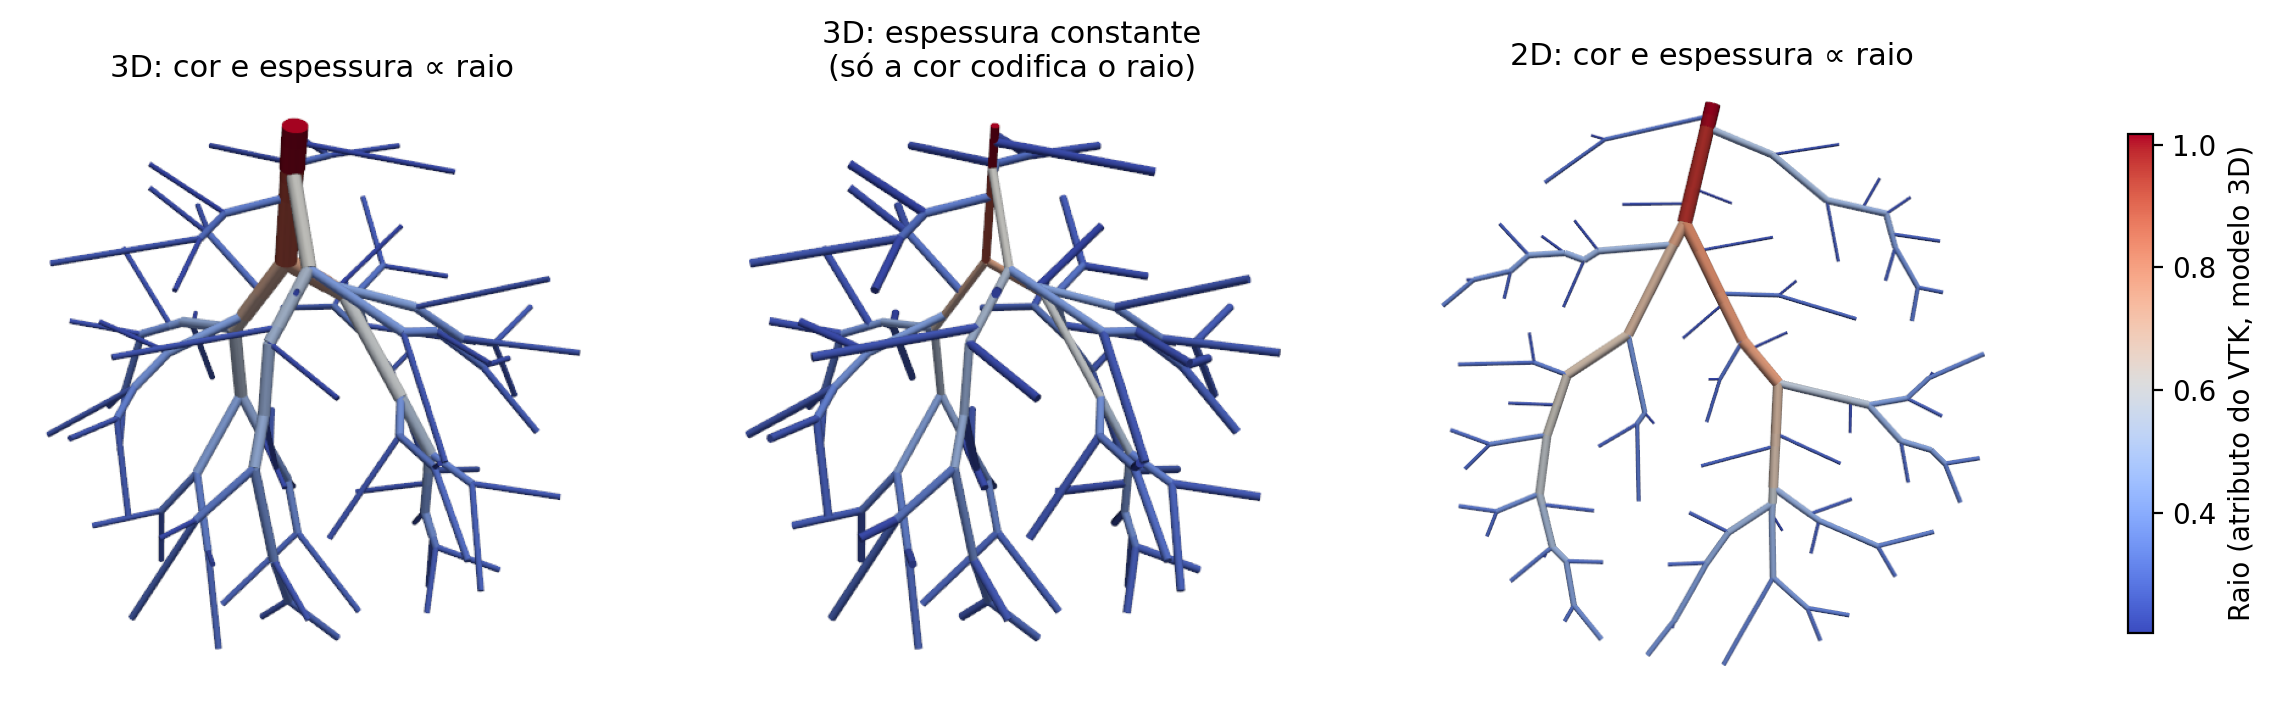
\includegraphics[width=\textwidth]{mod1_primitivas.png}
\caption{Módulo 1: tubos coloridos pelo raio (mapa \texttt{coolwarm}). Esquerda: modelo 3D com espessura proporcional ao raio; centro: espessura constante; direita: modelo 2D.}
\label{fig:mod1}
\end{figure}

\subsection{Módulo 2: transformações, vistas e projeções}
A Figura~\ref{fig:mod2t} mostra, com a câmera fixa, a árvore original e o resultado de uma translação, de uma rotação de $45^\circ$ e de uma escala uniforme de $1{,}1^5\approx1{,}61$. Como a câmera não se move, a mudança na imagem vem apenas da alteração das coordenadas no espaço do mundo. A Figura~\ref{fig:mod2v} mostra quatro posições do observador, e a Figura~\ref{fig:mod2p} compara as duas projeções com a mesma câmera. Na perspectiva, os ramos mais próximos do observador aparecem maiores e as retas paralelas convergem; na ortográfica, segmentos de mesmo comprimento aparecem iguais em qualquer profundidade, o que facilita comparar comprimentos e raios, mas tira a noção de profundidade.

\begin{figure}[H]
\centering
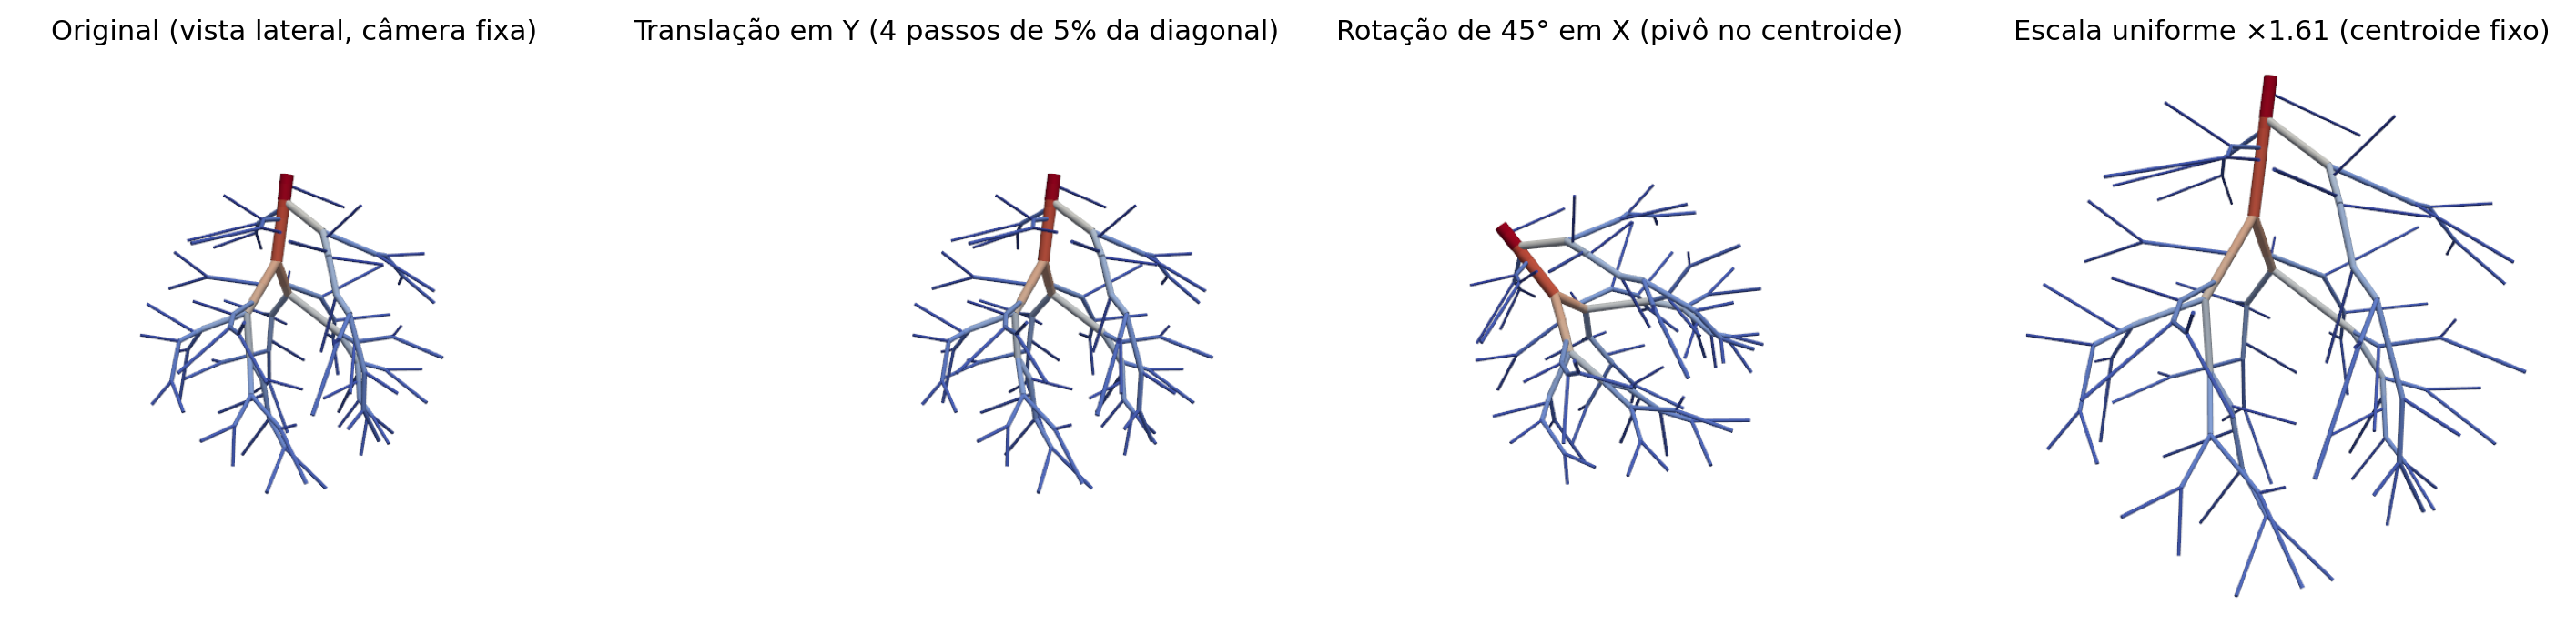
\includegraphics[width=\textwidth]{mod2_transformacoes.png}
\caption{Módulo 2: transformações aplicadas pelas matrizes $4\times4$ implementadas pelo grupo, com a câmera fixa (vista lateral).}
\label{fig:mod2t}
\end{figure}

\begin{figure}[H]
\centering
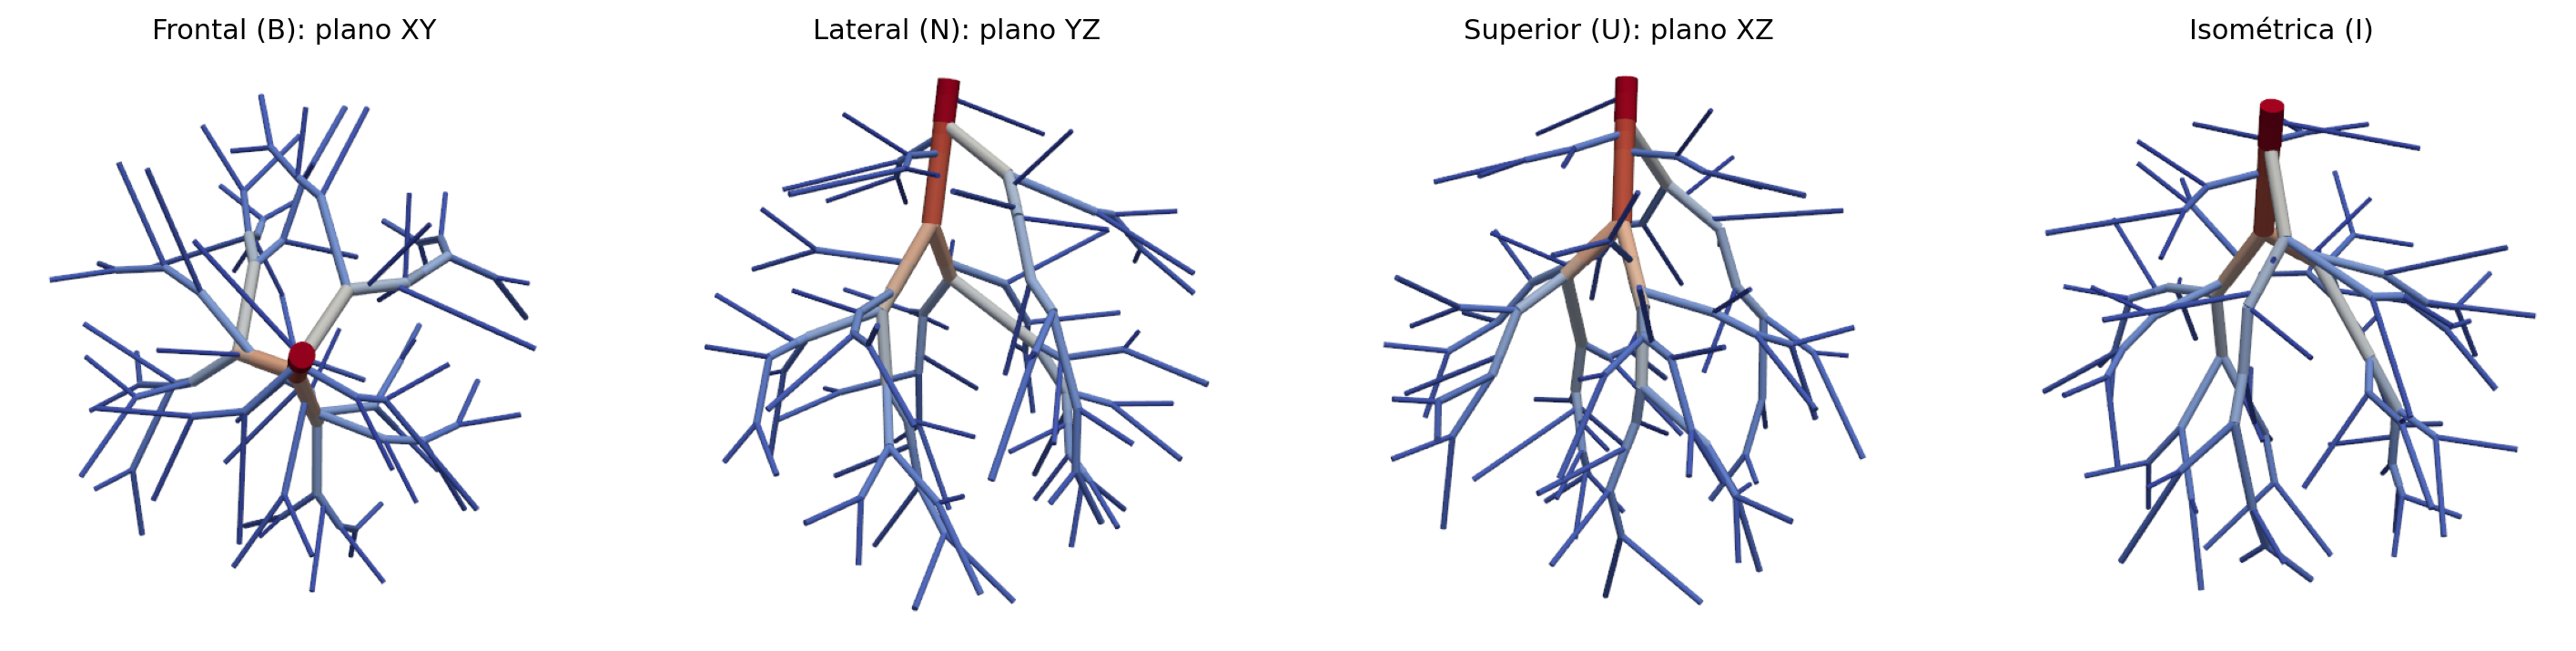
\includegraphics[width=\textwidth]{mod2_vistas.png}
\caption{Módulo 2: quatro posições do observador (teclas \texttt{B}, \texttt{N}, \texttt{U} e \texttt{I}).}
\label{fig:mod2v}
\end{figure}

\begin{figure}[H]
\centering
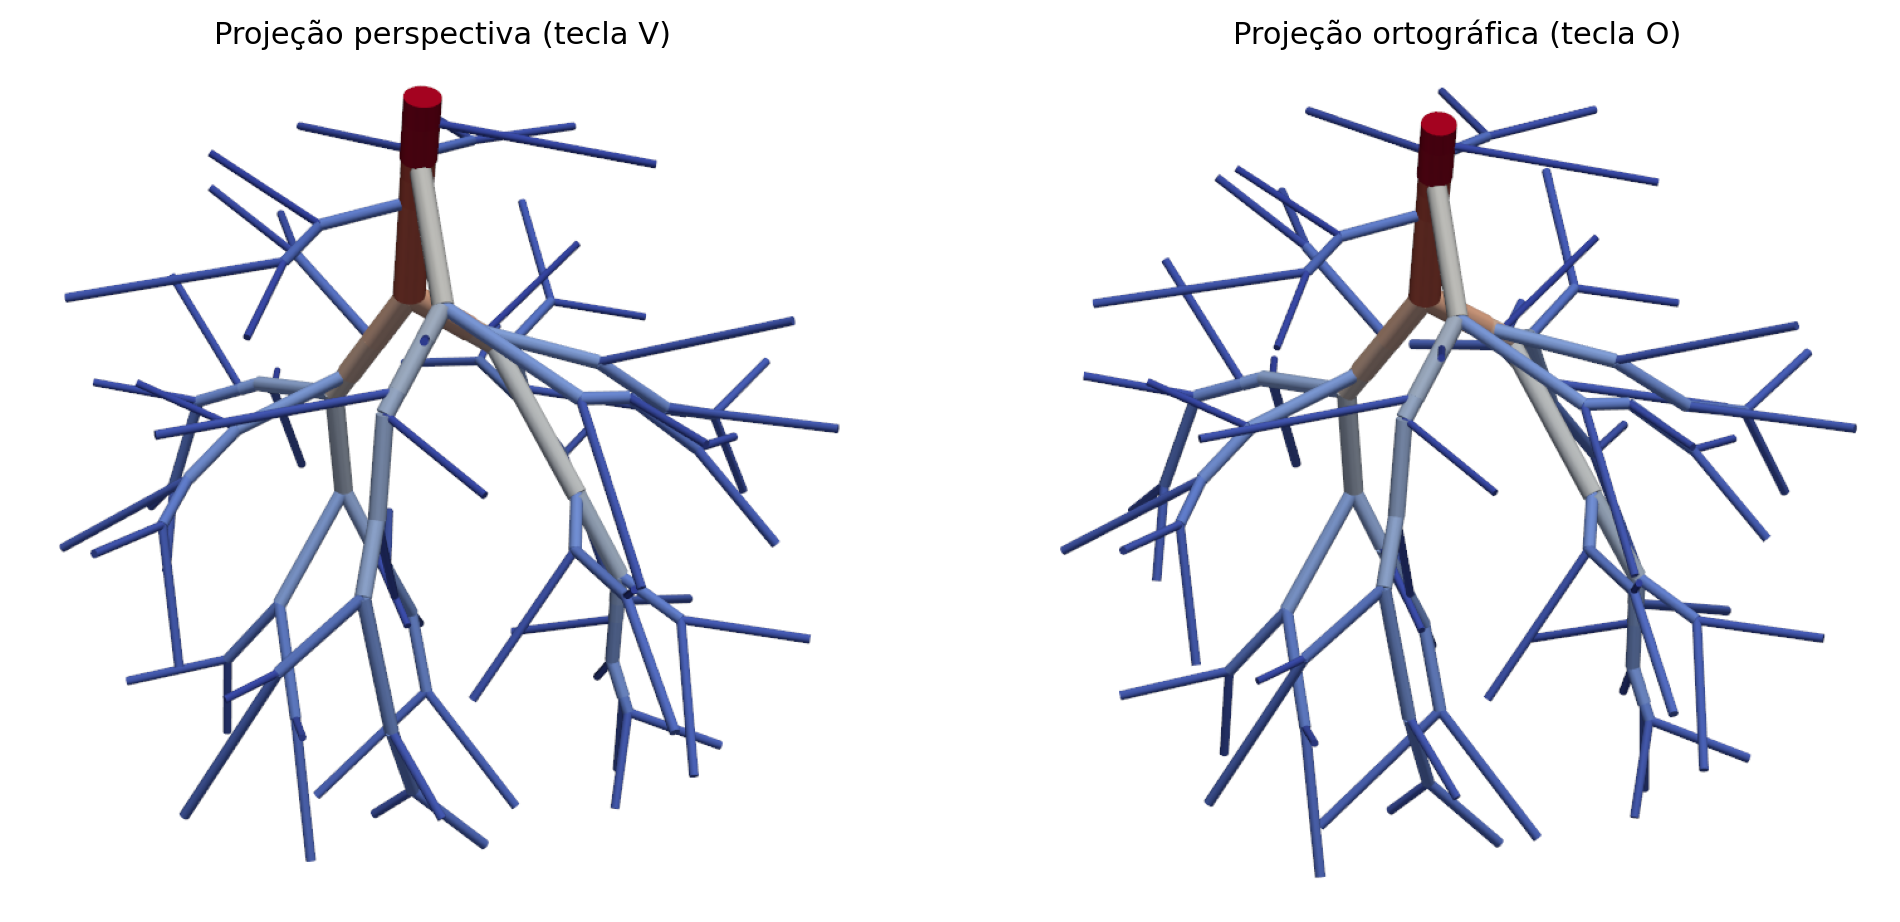
\includegraphics[width=0.82\textwidth]{mod2_projecoes.png}
\caption{Módulo 2: projeção perspectiva $\times$ ortográfica com a mesma posição de câmera.}
\label{fig:mod2p}
\end{figure}

\subsection{Módulo 3: rasterização de linhas}
A Tabela~\ref{tab:bres} mostra a execução do Bresenham de $(2,3)$ a $(14,10)$: $\Delta x=12$, $\Delta y=7$ e erro inicial $e=5$. São gerados $\max(12,7)+1=13$ pixels, e em cada coluna a distância vertical entre o centro do pixel escolhido e a reta ideal é de no máximo meio pixel (Figura~\ref{fig:mod3}, esquerda). À direita, os 127 segmentos da árvore 2D foram mapeados numa grade $60\times60$ com a mesma escala em $x$ e $y$ e rasterizados com a mesma função.

\begin{table}[H]
\centering\small
\caption{Execução do Bresenham de $(2,3)$ a $(14,10)$. A cada passo: avança $x$ se $e_2>-7$; avança $y$ se $e_2<12$.}
\label{tab:bres}
\setlength{\tabcolsep}{4pt}
\begin{tabular}{l*{13}{c}}
\toprule
\textbf{Passo} & 0 & 1 & 2 & 3 & 4 & 5 & 6 & 7 & 8 & 9 & 10 & 11 & 12 \\
\midrule
\textbf{Pixel} & (2,3) & (3,4) & (4,4) & (5,5) & (6,5) & (7,6) & (8,6) & (9,7) & (10,8) & (11,8) & (12,9) & (13,9) & (14,10) \\
$e$ & 5 & 10 & 3 & 8 & 1 & 6 & $-1$ & 4 & 9 & 2 & 7 & 0 & 5 \\
$e_2=2e$ & 10 & 20 & 6 & 16 & 2 & 12 & $-2$ & 8 & 18 & 4 & 14 & 0 & --- \\
\bottomrule
\end{tabular}
\end{table}

\begin{figure}[H]
\centering
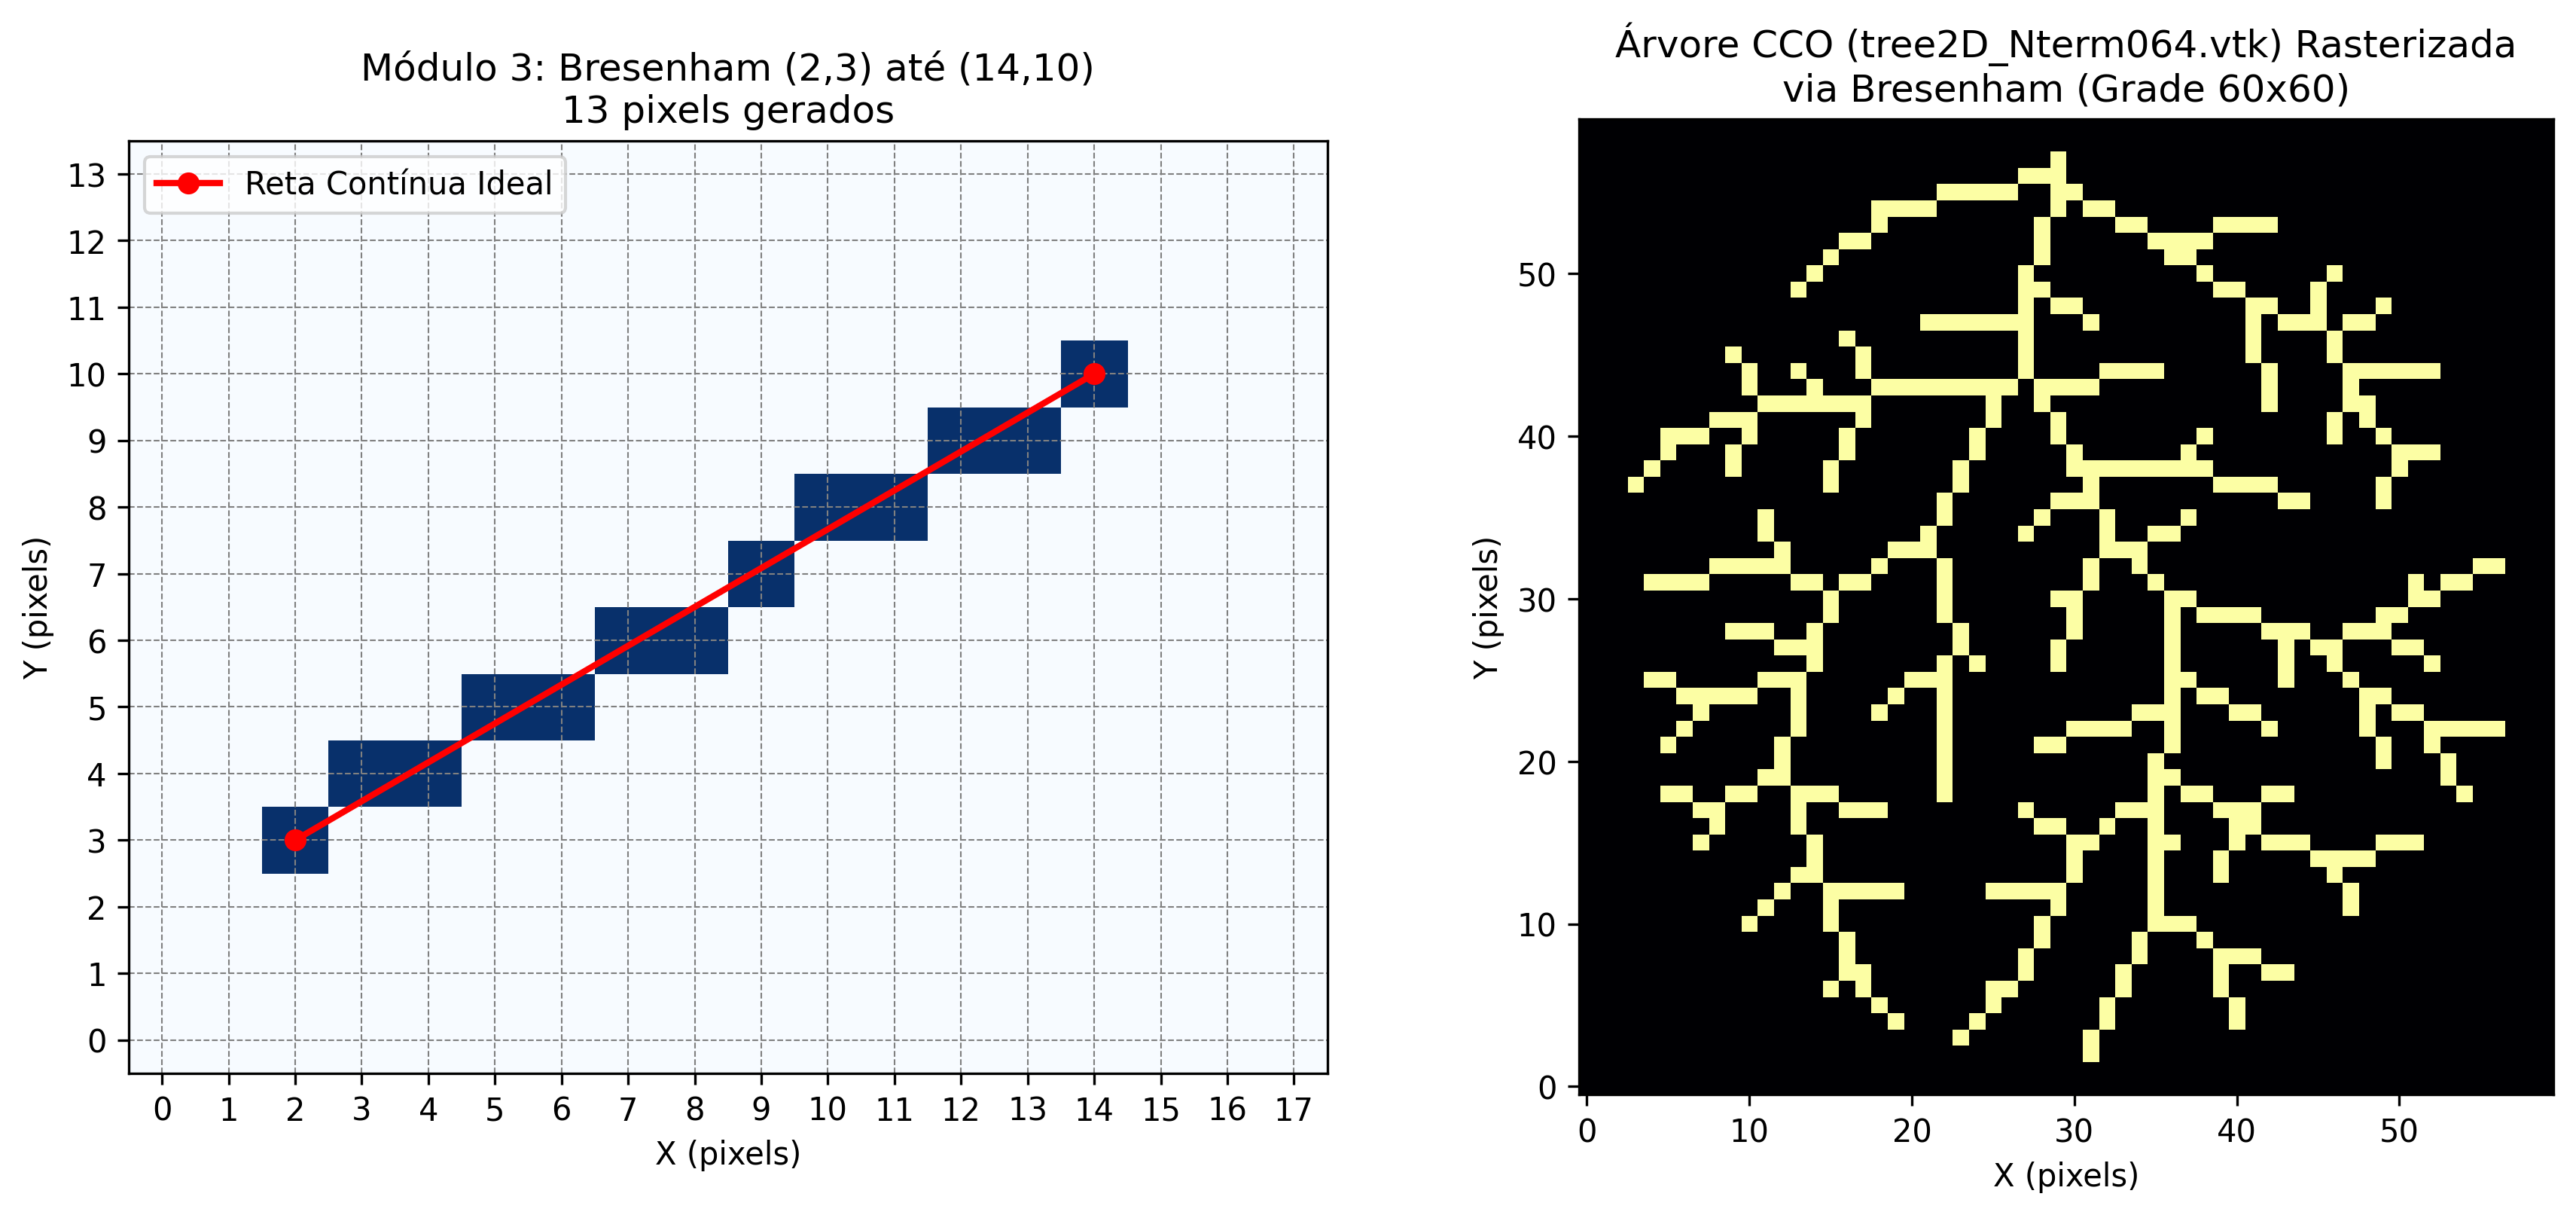
\includegraphics[width=0.92\textwidth]{mod3_bresenham.png}
\caption{Módulo 3: pixels gerados pelo Bresenham para o exemplo da Tabela~\ref{tab:bres} (esquerda) e para a árvore CCO 2D projetada numa grade $60\times60$ (direita).}
\label{fig:mod3}
\end{figure}

\subsection{Módulo 4: rasterização de polígonos}
O polígono de teste é côncavo, com seis vértices, e representa uma região de interesse. O Scanline com ET/AET preencheu 867 pixels nas linhas $y=6$ a $42$ (Figura~\ref{fig:mod4}). O painel do meio sobrepõe o contorno rasterizado por Bresenham, e o da direita compara as duas convenções de borda num quadrado $0..10$. A convenção fechada (pixels sobre o contorno incluídos) gera $11\times11=121$ pixels. A semiaberta (esquerda e base incluídas, direita e topo excluídos) gera $10\times10=100$ pixels; é a convenção usada para que polígonos vizinhos não pintem duas vezes os pixels da aresta comum.

\begin{figure}[H]
\centering
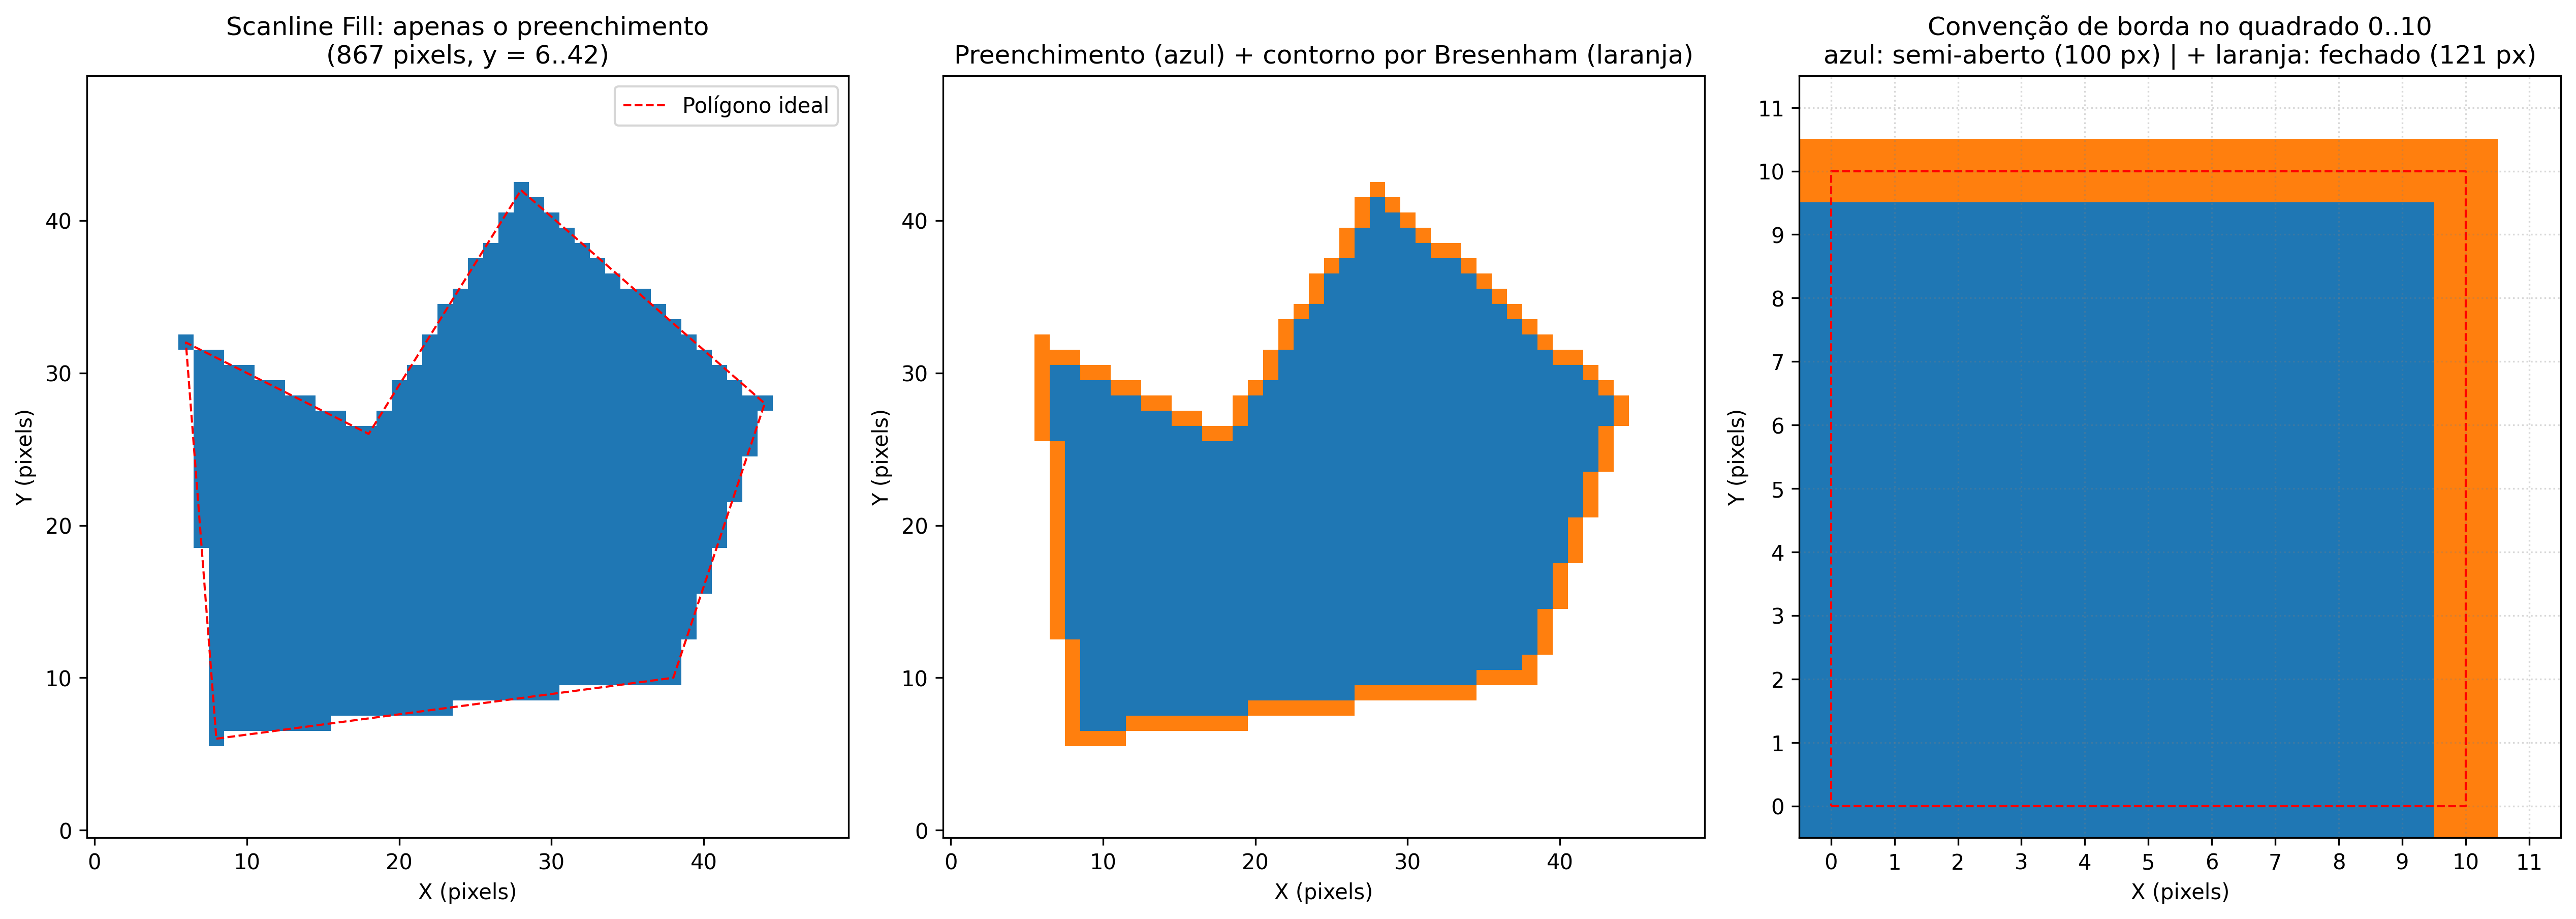
\includegraphics[width=\textwidth]{mod4_scanline.png}
\caption{Módulo 4: Scanline Fill de um polígono côncavo e convenções de borda.}
\label{fig:mod4}
\end{figure}

\subsection{Módulo 5: aliasing e antialiasing}
A Figura~\ref{fig:mod5} e a Tabela~\ref{tab:aa} comparam a rasterização da mesma geometria com 1, $2\times2$ e $4\times4$ amostras por pixel. Com uma amostra, cada pixel só pode valer 0 ou 1: a reta vira uma escada e, na árvore, vasos com menos de um pixel de largura se fragmentam em pontos isolados, porque o centro do pixel ora cai dentro, ora fora do traço. Com $k\times k$ amostras há $k^2+1$ níveis de intensidade, e o erro em relação à referência cai cerca de 11 vezes para a reta e 8 vezes para a árvore com $4\times4$ amostras. Os vasos finos aparecem como traços contínuos e mais claros, proporcionais à área que cobrem.

\begin{table}[H]
\centering\small
\caption{Níveis de intensidade e erro RMS em relação à referência $16\times16$.}
\label{tab:aa}
\begin{tabular}{lcccc}
\toprule
\textbf{Amostras por pixel} & \textbf{Níveis} & \textbf{Erro reta} & \textbf{Erro árvore} & \textbf{Custo relativo} \\
\midrule
1 (sem AA) & 2 & 0,0797 & 0,1206 & 1$\times$ \\
$2\times2$ (SSAA) & 5 & 0,0229 & 0,0443 & 4$\times$ \\
$4\times4$ (SSAA) & 17 & 0,0073 & 0,0154 & 16$\times$ \\
\bottomrule
\end{tabular}
\end{table}

\begin{figure}[H]
\centering
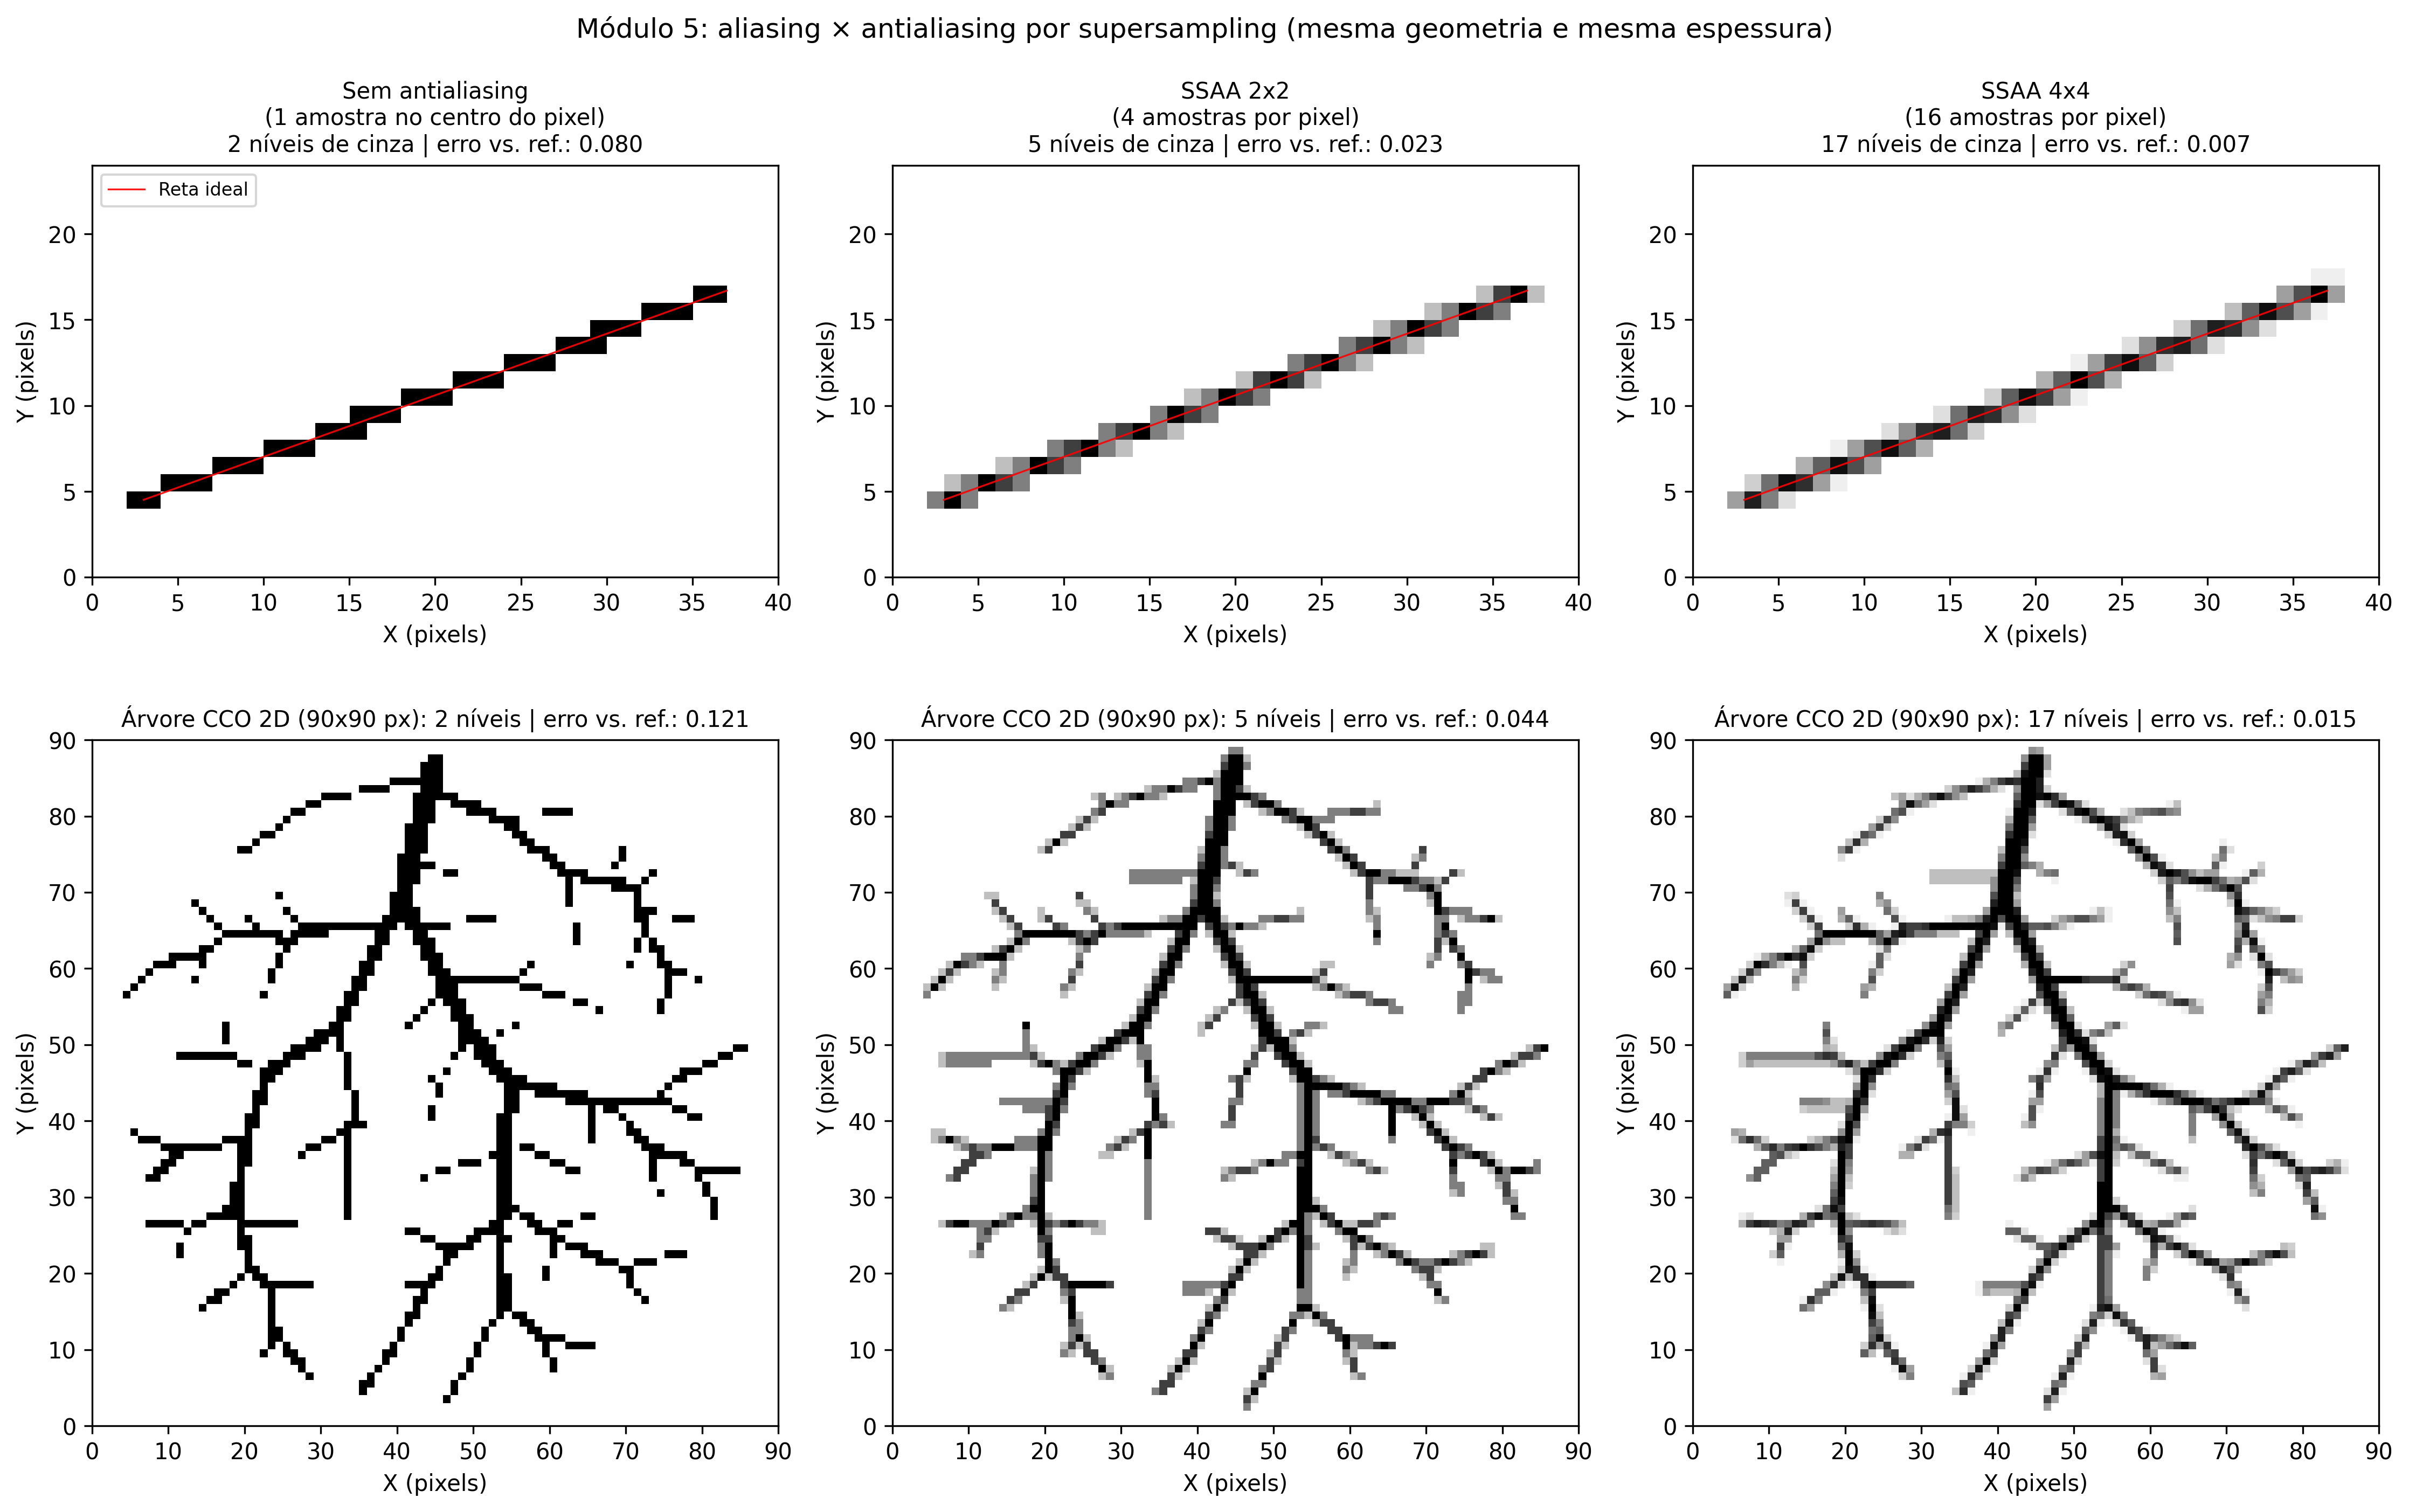
\includegraphics[width=\textwidth]{mod5_antialiasing.png}
\caption{Módulo 5: supersampling implementado pelo grupo. Linha superior: segmento inclinado; linha inferior: árvore 2D a $90\times90$ pixels, com espessura proporcional ao raio.}
\label{fig:mod5}
\end{figure}

No visualizador, a tecla \texttt{A} alterna entre sem antialiasing, MSAA e SSAA, fornecidos pelo VTK. A Figura~\ref{fig:mod5v} amplia uma região da imagem: sem antialiasing, as bordas dos tubos inclinados formam degraus; com MSAA e SSAA, os pixels de borda recebem cores intermediárias entre o tubo e o fundo.

\begin{figure}[H]
\centering
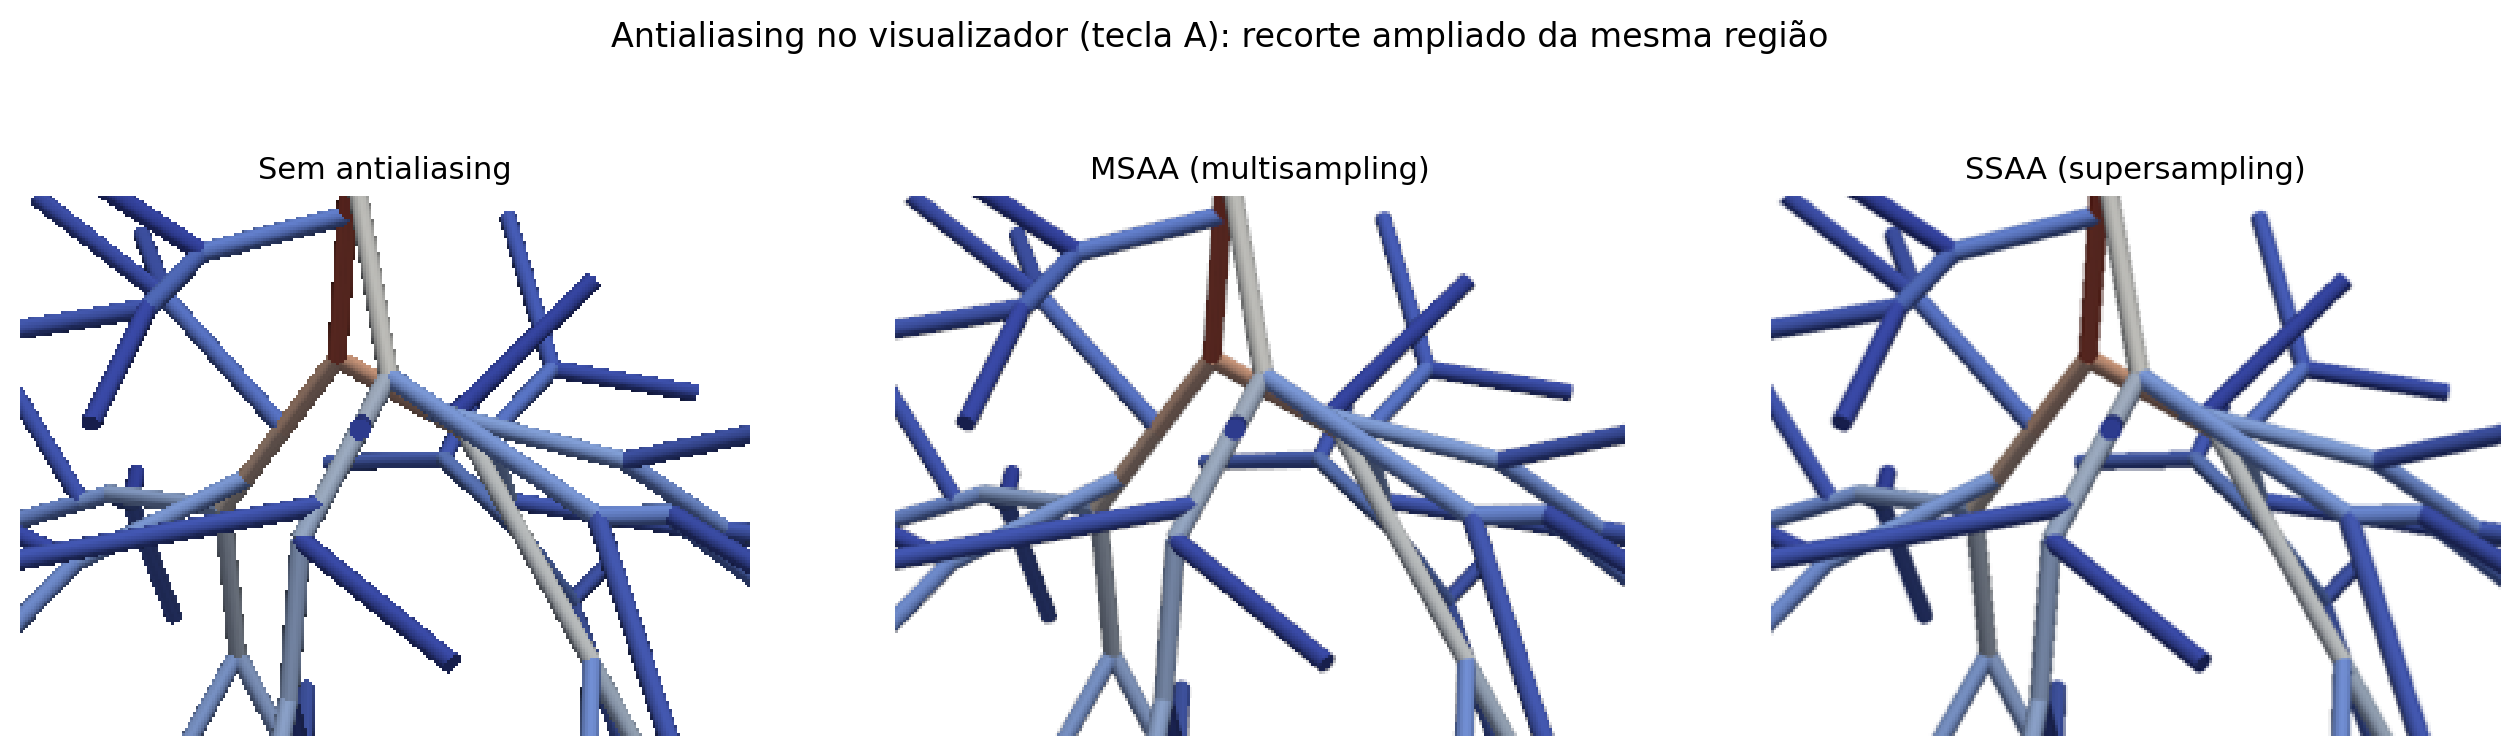
\includegraphics[width=\textwidth]{mod5_viewer_aa.png}
\caption{Módulo 5: antialiasing da API no visualizador 3D (mesma região ampliada).}
\label{fig:mod5v}
\end{figure}

\subsection{Módulo 6: recorte de segmentos}
Os 127 segmentos da árvore 2D foram recortados pela janela $[-0{,}022;\,0{,}022]\times[-0{,}020;\,0{,}025]$. A Figura~\ref{fig:mod6} mostra a árvore antes do recorte e o resultado de cada algoritmo: os dois deixam 35 segmentos visíveis, e a comparação ponto a ponto não encontrou nenhuma divergência. Segmentos que apenas tocam a janela num ponto são descartados por ambos. A Figura~\ref{fig:mod6c} e a Tabela~\ref{tab:clip} comparam o custo.

\begin{figure}[H]
\centering
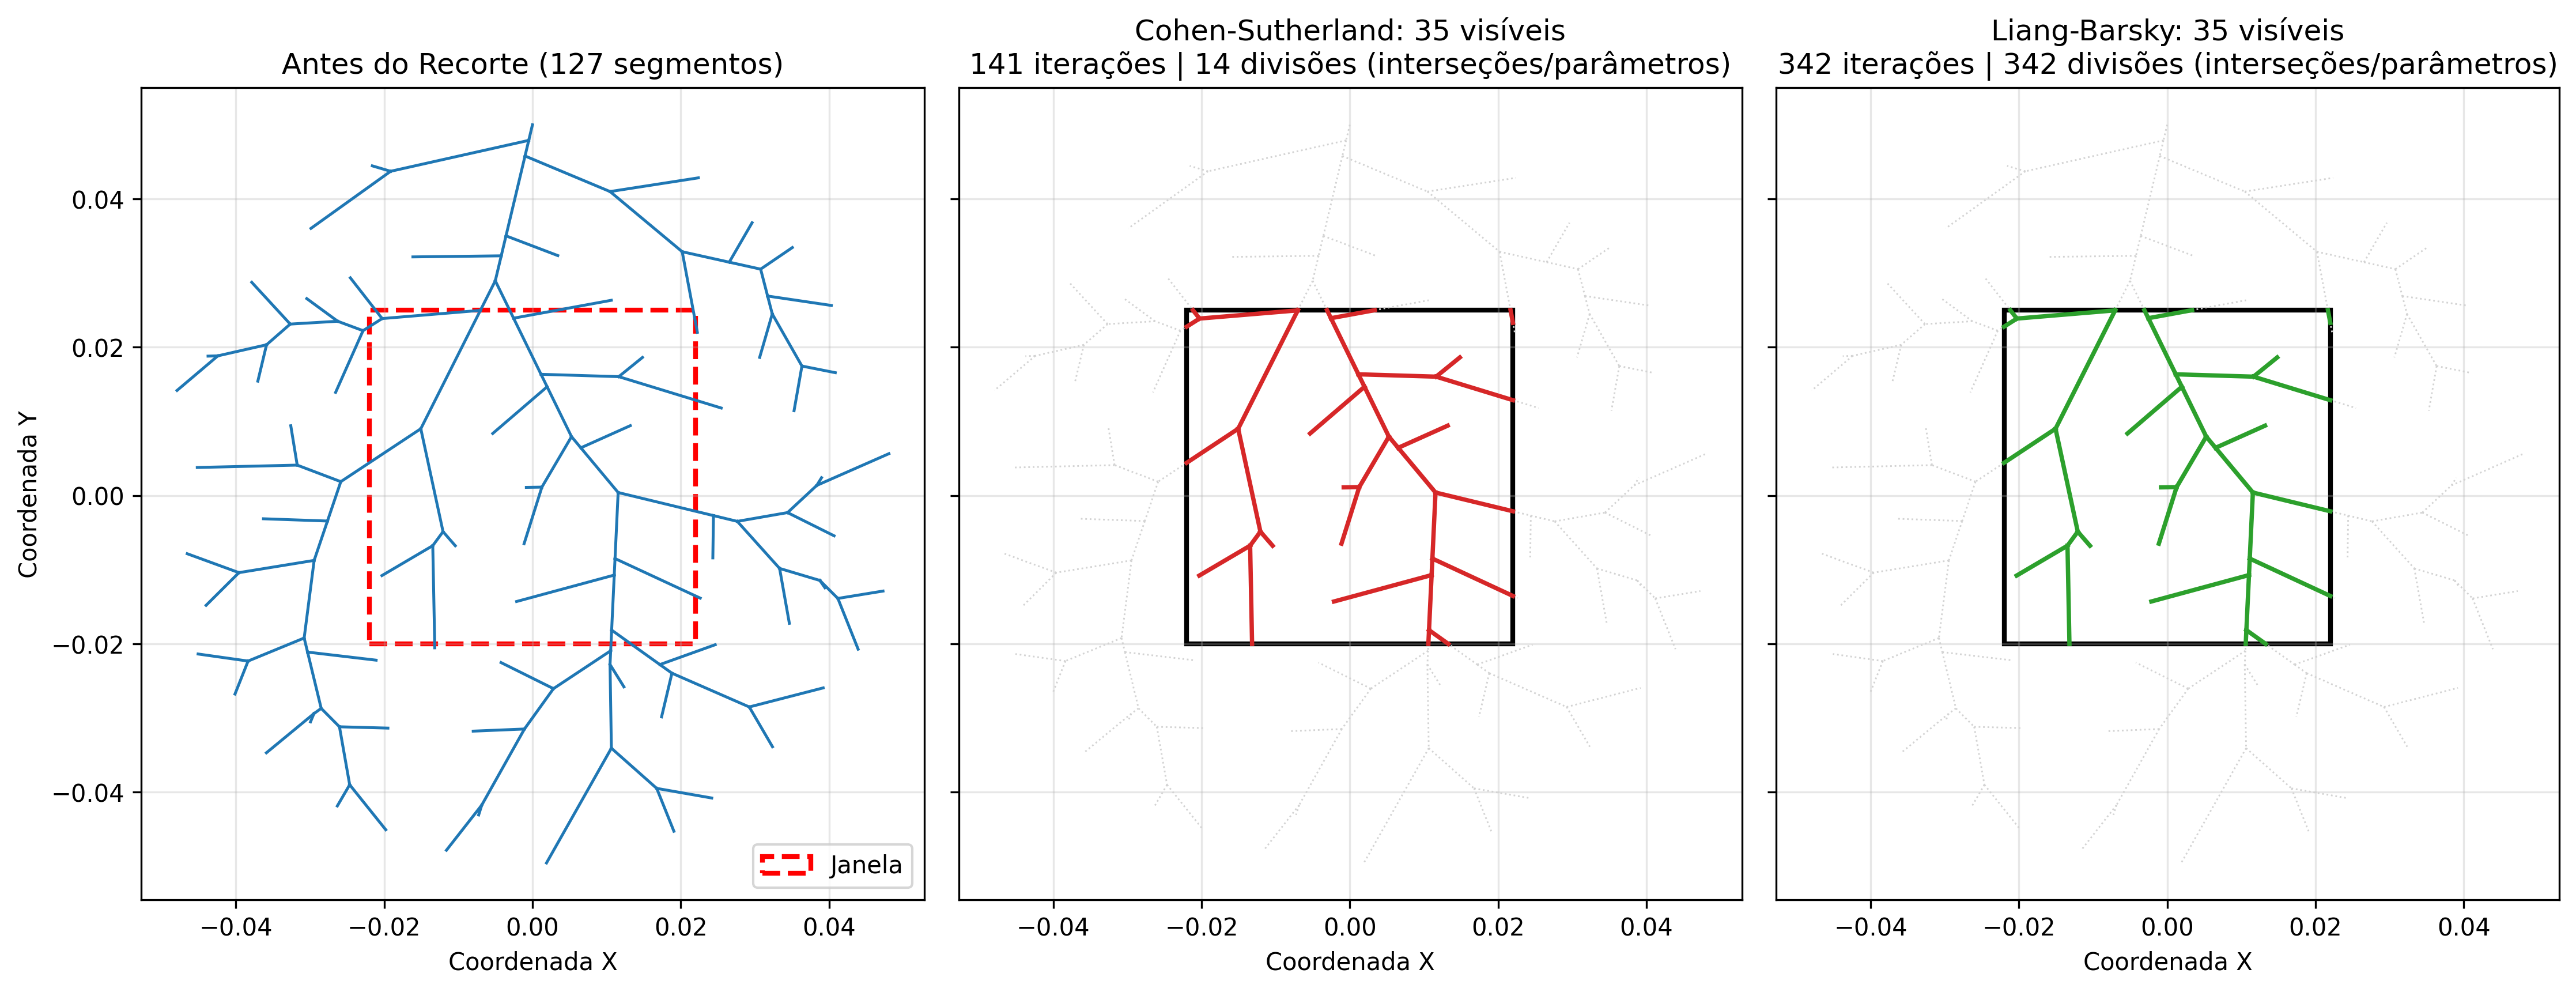
\includegraphics[width=\textwidth]{mod6_line_clipping.png}
\caption{Módulo 6: árvore 2D antes do recorte e resultados de Cohen--Sutherland e Liang--Barsky.}
\label{fig:mod6}
\end{figure}

\begin{table}[H]
\centering\small
\caption{Custo do recorte dos 127 segmentos. ``Iteração'' é uma passada do laço (CS) ou um teste de borda (LB). O tempo é a média de 300 repetições em Python e depende da máquina.}
\label{tab:clip}
\begin{tabular}{lcccc}
\toprule
\textbf{Algoritmo} & \textbf{Visíveis} & \textbf{Iterações} & \textbf{Divisões} & \textbf{Tempo/segmento} \\
\midrule
Cohen--Sutherland & 35 & 141 & 14 & 2,25\,$\mu$s \\
Liang--Barsky & 35 & 342 & 342 & 3,38\,$\mu$s \\
\bottomrule
\end{tabular}
\end{table}

\begin{figure}[H]
\centering
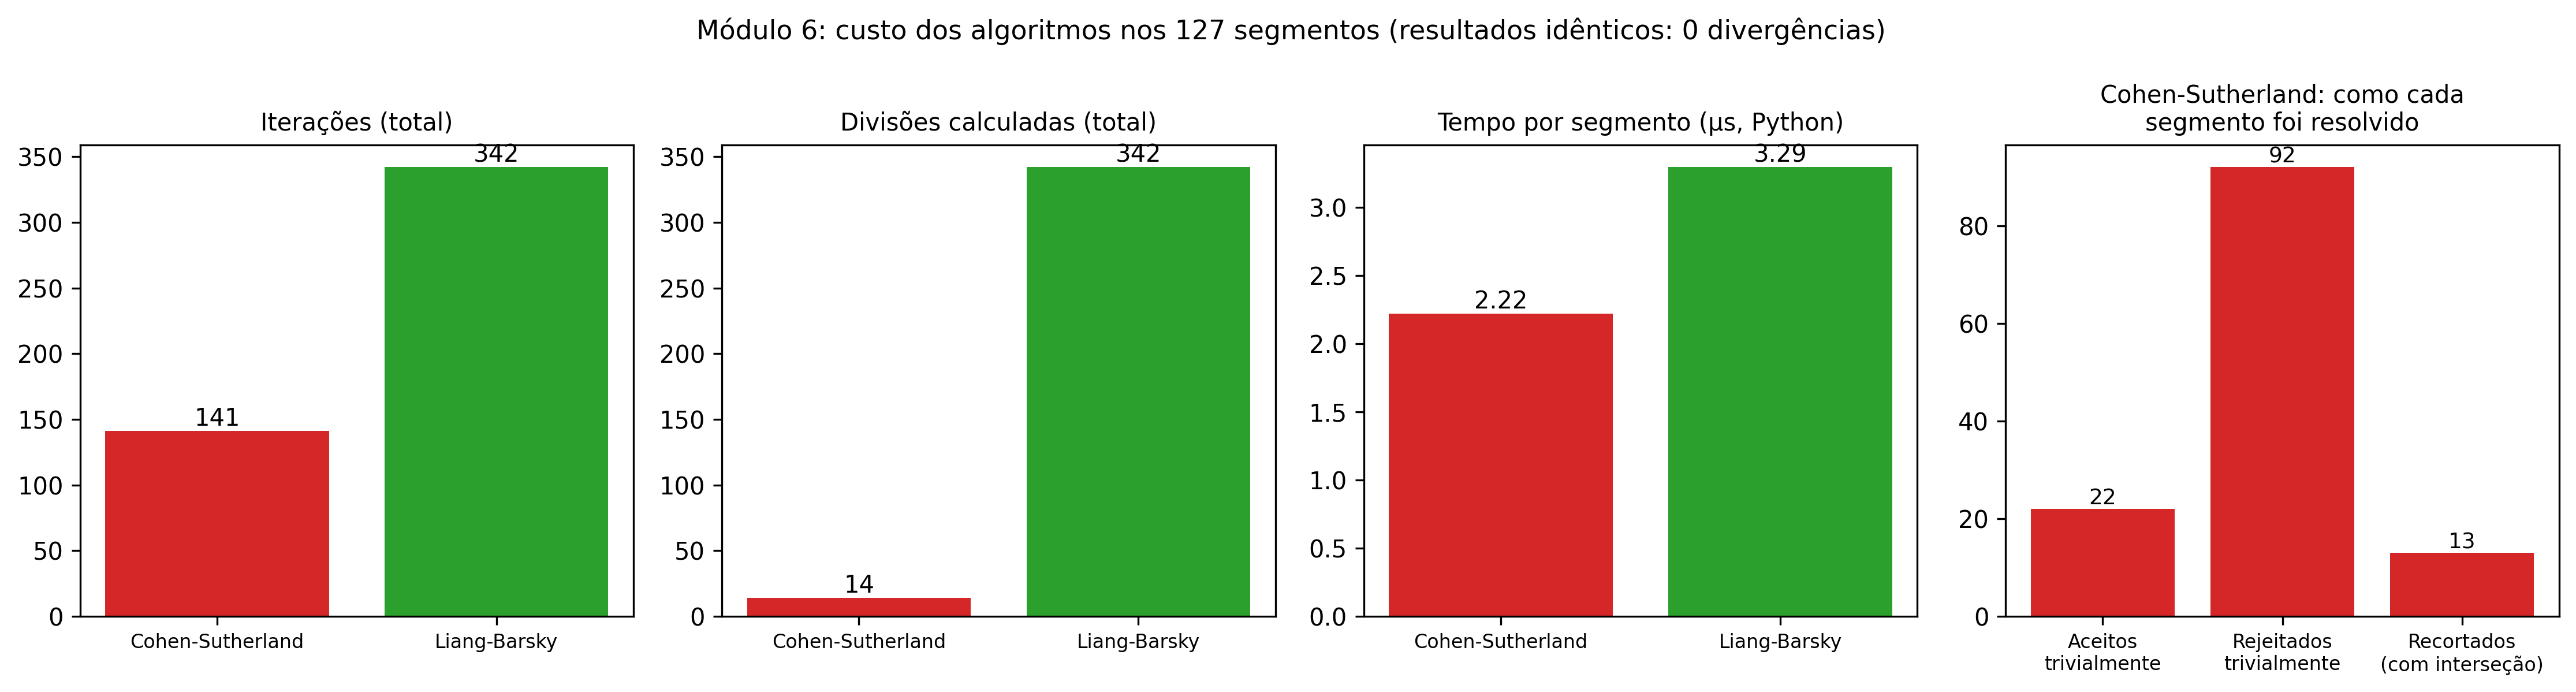
\includegraphics[width=\textwidth]{mod6_comparacao_algoritmos.png}
\caption{Módulo 6: custo dos dois algoritmos e classificação dos segmentos pelo Cohen--Sutherland (22 aceitos e 92 rejeitados trivialmente, 13 recortados).}
\label{fig:mod6c}
\end{figure}

\subsection{Módulo 7: recorte de polígonos}
Na Figura~\ref{fig:mod7} (acima), um polígono de 7 vértices que ultrapassa os quatro lados da janela $[0,10]^2$ foi recortado pelo Sutherland--Hodgman, resultando em um polígono de 8 vértices; a mesma janela em sentido horário é reorientada automaticamente e produz o mesmo resultado. Abaixo, um polígono côncavo em forma de ``U'' é recortado pela faixa $5\le y\le10$. O resultado correto são duas regiões (os dois braços), mas o algoritmo devolve uma única lista de 8 vértices, ligando os braços por duas arestas sobrepostas de comprimento 4 ao longo de $y=5$ (destacadas em vermelho). Se esse polígono fosse preenchido ou tivesse o contorno desenhado, apareceria um traço falso entre os braços. É o caso em que o Weiler--Atherton é o algoritmo adequado.

\begin{figure}[H]
\centering
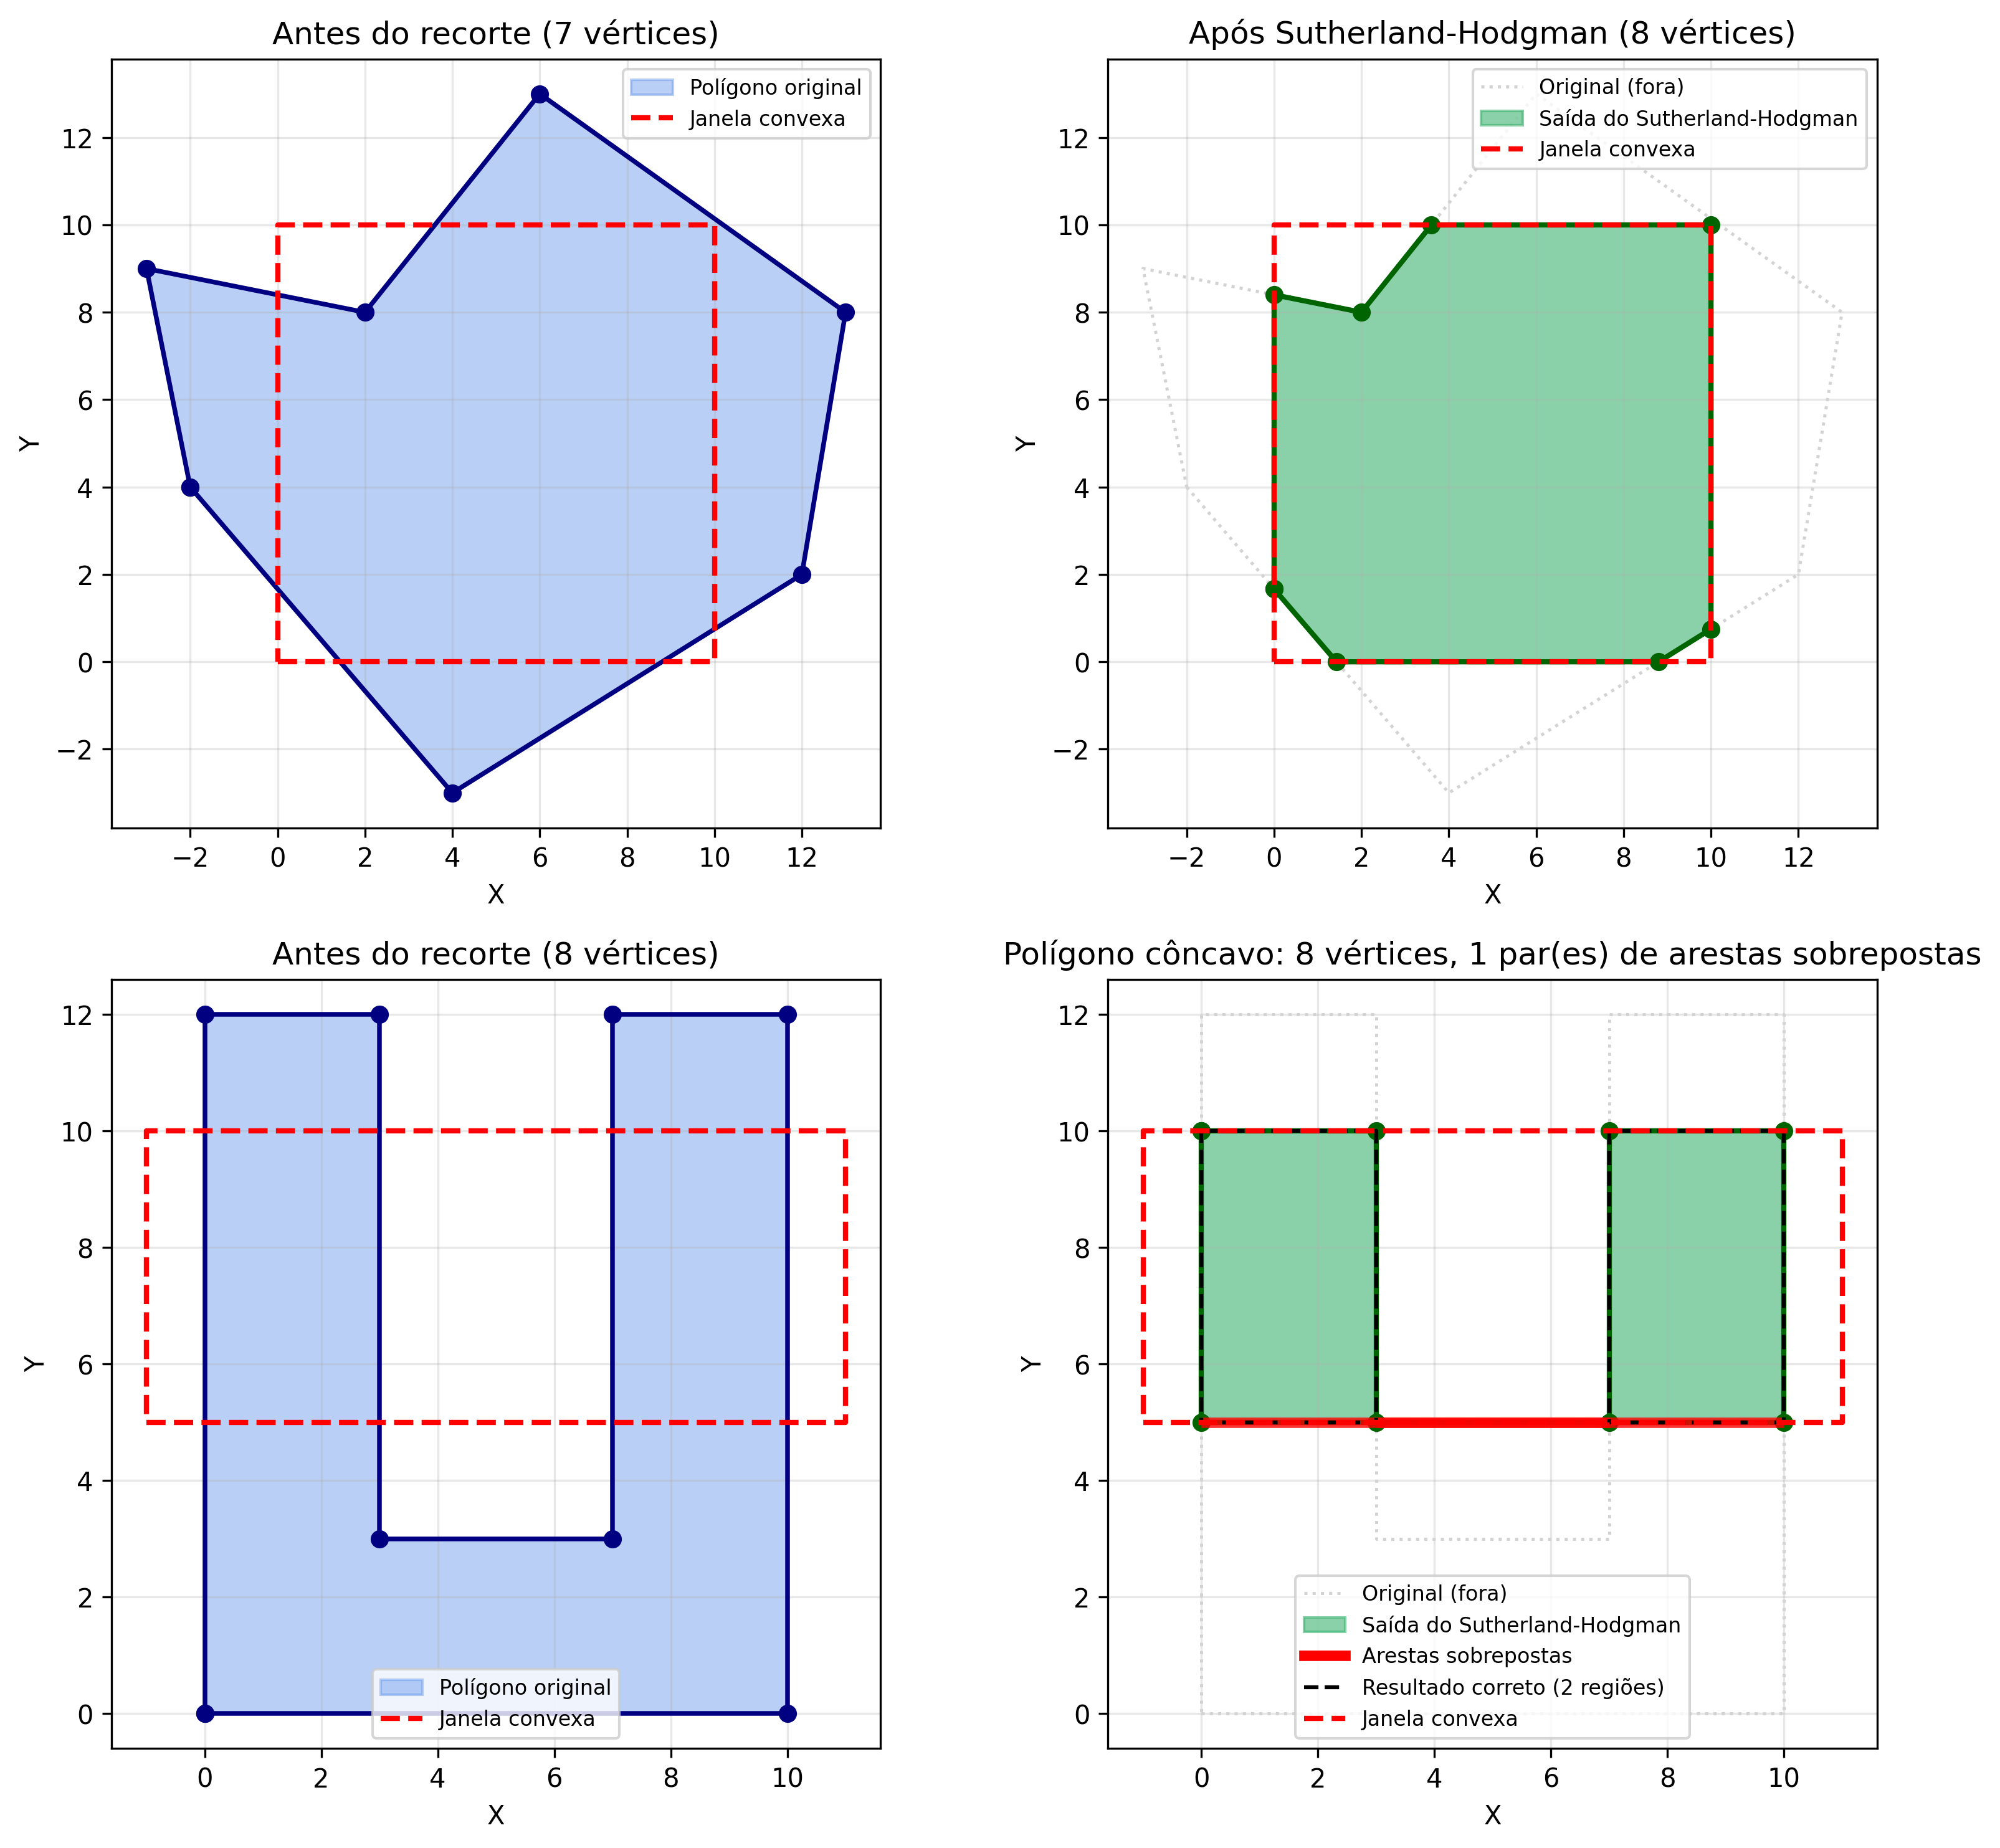
\includegraphics[width=0.78\textwidth]{mod7_polygon_clipping.png}
\caption{Módulo 7: Sutherland--Hodgman num polígono qualquer (acima) e num polígono côncavo cujo recorte correto tem duas regiões (abaixo).}
\label{fig:mod7}
\end{figure}

% =====================================================================
\section{Discussão}\label{sec:disc}
% =====================================================================
\textbf{Comparação entre algoritmos de recorte.} Na árvore CCO a maioria dos segmentos é curta em relação à janela, então quase todos ficam inteiramente dentro ou do mesmo lado de fora. O Cohen--Sutherland resolveu 114 dos 127 segmentos (90\%) apenas com operações de bits, sem nenhuma divisão, e calculou só 14 interseções. O Liang--Barsky sempre executa os quatro testes de borda e calcula até quatro razões $q_k/p_k$ por segmento, totalizando 342 divisões; nesta cena ele foi cerca de 1,5 vez mais lento. A vantagem do Liang--Barsky aparece quando muitos segmentos cruzam a janela: o Cohen--Sutherland pode então calcular interseções intermediárias que serão descartadas (um extremo é movido para uma borda e ainda fica fora), enquanto o Liang--Barsky calcula cada extremo final uma única vez. O Cyrus--Beck, por sua vez, só se justifica quando a janela não é um retângulo alinhado aos eixos.

\textbf{Decisões de implementação.} (i) Um tubo por segmento, com pontos duplicados, para que o raio não seja interpolado entre vasos vizinhos. (ii) O pivô das transformações é o centroide atual, para que a árvore gire e escale ``no lugar'' e para que cada operação tenha inversa exata. (iii) Na comparação de antialiasing, a geometria e a espessura são idênticas nos três casos e só muda o número de amostras; assim a diferença nas imagens vem apenas da amostragem. (iv) O Scanline usa intervalos semiabertos em $y$ para tratar vértices compartilhados e arestas horizontais sem casos especiais; a versão fechada é a união de duas passadas, uma delas com o polígono espelhado em $y$. (v) O Sutherland--Hodgman valida que a janela é convexa e não degenerada e a reorienta para o sentido anti-horário, pois o teste de lado interno depende da orientação.

\textbf{Limitações.} O recorte e a rasterização didáticos operam sobre a projeção 2D (plano $XY$), e não dentro do \emph{pipeline} 3D, onde o recorte é feito pela GPU contra o volume de visualização em coordenadas homogêneas. A malha de tubos é reconstruída a cada transformação, o que é aceitável para 127 segmentos, mas não escalaria para árvores com milhares de terminais; nesse caso a matriz deveria ser aplicada ao ator (\texttt{user\_matrix}) ou na GPU. O Weiler--Atherton e o Cyrus--Beck foram apenas discutidos. As bifurcações não recebem esferas de junção, o que deixa pequenas descontinuidades entre tubos de raios muito diferentes.

% =====================================================================
\section{Conclusão}
% =====================================================================
Desenvolvemos uma aplicação que cobre os sete módulos do TP1 sobre os modelos CCO fornecidos: leitura própria do VTK, representação por tubos com cor e espessura proporcionais ao raio, transformações com matrizes homogêneas, quatro vistas e duas projeções, Bresenham, Scanline com ET/AET, supersampling, Cohen--Sutherland, Liang--Barsky e Sutherland--Hodgman. As partes implementadas pelo grupo e as fornecidas pelo PyVista/VTK estão separadas no código e na Tabela~\ref{tab:modulos}. Os experimentos quantificaram o ganho do supersampling, mostraram que os dois algoritmos de recorte de segmentos produzem o mesmo resultado com custos diferentes e evidenciaram a limitação do Sutherland--Hodgman com polígonos côncavos. Como trabalho futuro, no TP2, a mesma base receberá visibilidade (Z-buffer), modelos de iluminação, transparência e técnicas baseadas em raios, como a seleção de vasos por \emph{ray casting}.

% --- AGRADECIMENTOS ---
\section*{Agradecimentos}
Os autores agradecem ao Departamento de Computação (DECOM) da Universidade Federal de Ouro Preto (UFOP) e ao professor da disciplina pelos modelos CCO disponibilizados.

% --- REFERÊNCIAS BIBLIOGRÁFICAS ---
\begin{thebibliography}{99}
  \bibitem{schreiner1993} SCHREINER, W.; BUXBAUM, P. F. Computer-optimization of vascular trees. \textbf{IEEE Transactions on Biomedical Engineering}, v. 40, n. 5, p. 482--491, 1993.
  \bibitem{foley} FOLEY, J. D.; VAN DAM, A.; FEINER, S. K.; HUGHES, J. F. \textbf{Computer Graphics: Principles and Practice}. 2. ed. Reading: Addison-Wesley, 1996.
  \bibitem{hearn} HEARN, D.; BAKER, M. P.; CARITHERS, W. \textbf{Computer Graphics with OpenGL}. 4. ed. Boston: Pearson, 2011.
  \bibitem{angel} ANGEL, E.; SHREINER, D. \textbf{Interactive Computer Graphics: A Top-Down Approach with WebGL}. 7. ed. Boston: Pearson, 2015.
  \bibitem{bresenham1965} BRESENHAM, J. E. Algorithm for computer control of a digital plotter. \textbf{IBM Systems Journal}, v. 4, n. 1, p. 25--30, 1965.
  \bibitem{liang1984} LIANG, Y.-D.; BARSKY, B. A. A new concept and method for line clipping. \textbf{ACM Transactions on Graphics}, v. 3, n. 1, p. 1--22, 1984.
  \bibitem{cyrus1978} CYRUS, M.; BECK, J. Generalized two- and three-dimensional clipping. \textbf{Computers \& Graphics}, v. 3, n. 1, p. 23--28, 1978.
  \bibitem{sutherland1974} SUTHERLAND, I. E.; HODGMAN, G. W. Reentrant polygon clipping. \textbf{Communications of the ACM}, v. 17, n. 1, p. 32--42, 1974.
  \bibitem{weiler1977} WEILER, K.; ATHERTON, P. Hidden surface removal using polygon area sorting. \textbf{ACM SIGGRAPH Computer Graphics}, v. 11, n. 2, p. 214--222, 1977.
  \bibitem{vtk} SCHROEDER, W.; MARTIN, K.; LORENSEN, B. \textbf{The Visualization Toolkit}. 4. ed. Kitware, 2006. Disponível em: \url{https://vtk.org/}.
  \bibitem{pyvista} SULLIVAN, C. B.; KASZYNSKI, A. PyVista: 3D plotting and mesh analysis through a streamlined interface for the Visualization Toolkit (VTK). \textbf{Journal of Open Source Software}, v. 4, n. 37, p. 1450, 2019.
\end{thebibliography}

\end{document}
